\documentclass[compress]{beamer}
\usepackage{ifthen,verbatim}

\newcommand{\isnote}{}
\xdefinecolor{lightyellow}{rgb}{1.,1.,0.25}
\xdefinecolor{darkblue}{rgb}{0.1,0.1,0.7}
\xdefinecolor{darkgreen}{rgb}{0.,0.5,0.}

%% Uncomment this to get annotations
%% \def\notes{\addtocounter{page}{-1}
%%            \renewcommand{\isnote}{*}
%% 	   \beamertemplateshadingbackground{lightyellow}{white}
%%            \begin{frame}
%%            \frametitle{Notes for the previous page (page \insertpagenumber)}
%%            \itemize}
%% \def\endnotes{\enditemize
%% 	      \end{frame}
%%               \beamertemplateshadingbackground{white}{white}
%%               \renewcommand{\isnote}{}}

%% Uncomment this to not get annotations
\def\notes{\comment}
\def\endnotes{\endcomment}

\setbeamertemplate{navigation symbols}{}
\setbeamertemplate{headline}{\mbox{ } \hfill
\begin{minipage}{5.5 cm}
\vspace{-0.75 cm} \small
\end{minipage} \hfill
\begin{minipage}{4.5 cm}
\vspace{-0.75 cm} \small
\begin{flushright}
\ifthenelse{\equal{\insertpagenumber}{1}}{}{Jim Pivarski \hspace{0.2 cm} \insertpagenumber\isnote/\pageref{numpages}}
\end{flushright}
\end{minipage}\mbox{\hspace{0.2 cm}}\includegraphics[height=1 cm]{../cmslogo} \hspace{0.1 cm} \includegraphics[height=1 cm]{../tamulogo} \hspace{0.01 cm} \vspace{-1.05 cm}}

\begin{document}
\begin{frame}
\vfill
\begin{center}
\textcolor{darkblue}{\Large Alignment with Tracks}

\vfill
\begin{columns}
\column{0.3\linewidth}
\begin{center}
\large
\textcolor{darkblue}{Jim Pivarski}

\vspace{0.2 cm}
Alexei Safonov
\end{center}
\end{columns}

\begin{columns}
\column{0.3\linewidth}
\begin{center}
\scriptsize
{\it Texas A\&M University}
\end{center}
\end{columns}

\vfill
21 June, 2009

\end{center}
\end{frame}

%% \begin{notes}
%% \item This is the annotated version of my talk.
%% \item If you want the version that I am presenting, download the one
%% labeled ``slides'' on Indico (or just ignore these yellow pages).
%% \item The annotated version is provided for extra detail and a written
%% record of comments that I intend to make orally.
%% \item Yellow notes refer to the content on the {\it previous} page.
%% \item All other slides are identical for the two versions.
%% \end{notes}

\small

\section*{Introduction}

\begin{frame}
\frametitle{Outline for this talk}
\begin{itemize}\setlength{\itemsep}{0.75 cm}
\item Reminder of pre-collisions goals, status of procedures and constants
\item What we learned from beam-halo/CRAFT and how it applies to collisions data
\item Timeline of what needs to be done when the beam arrives
\end{itemize}
%% \hspace{-0.83 cm} \textcolor{darkblue}{\Large Outline2}
\end{frame}

\begin{frame}
\frametitle{Goals for pre-collisions}
\begin{itemize}
\item \textcolor{darkblue}{Primary:} test and improve all parts of the
  alignment system, \\ with a strong preference for procedures that will
  be useful in the colliding-beams era
\item \textcolor{darkblue}{Secondary:} develop new procedures that are
  better optimized for cosmic rays, to improve constants more now
\end{itemize}

\scriptsize
\hspace{4.3 cm}\textcolor{darkblue}{$^*$Applicable to\ldots}

\vspace{-0.17 cm}
\mbox{\hspace{-0.6 cm}\begin{minipage}{\linewidth}
\renewcommand{\arraystretch}{2}
\begin{tabular}{c p{0.2\linewidth} p{1.5 cm} p{1.5 cm} p{1.5 cm}p{0.25\linewidth}}
& \textcolor{darkblue}{Procedure} & \textcolor{darkblue}{collisions} & \textcolor{darkblue}{beam-halo} & \textcolor{darkblue}{cosmics} & \textcolor{darkblue}{Status} \\\hline
1. & CSC Overlaps & \textcolor{red}{yes} & \textcolor{red}{yes} & no & \textcolor{black}{validated~with~data} (ME$-$2/1,~$-$3/1) \\
2. & Tracker-to-muon chambers (``Baseline'') & \textcolor{red}{yes} & no & \textcolor{red}{DT~wheels $-$1,~0,~$+$1} & \textcolor{black}{validated with data, provided constants, sub-mm precision} \\
3. & Tracker-to-CSC disk & \textcolor{red}{yes} & no & \textcolor{red}{seems to be possible, but rough} & \textcolor{black}{observing~first~results, \mbox{provided~constants,}} needs~more~work \\
4. & Barrel-to-endcap & no & no & \textcolor{red}{yes} & in development \\
\end{tabular}
\end{minipage}}

\vspace{0.25 cm}
\textcolor{darkblue}{$^*$Depends on track distributions: beamspot-pointing, longitudinal, and mostly vertical\hspace{-1 cm}}
\end{frame}

\section*{1. CSC Overlaps}
\begin{frame}
\begin{center}
\Huge \textcolor{blue}{1. CSC Overlaps}
\end{center}
\end{frame}

\begin{frame}
\frametitle{1. CSC Overlaps}
\vspace{0.2 cm}
\begin{columns}
\column{0.5\linewidth}
\vspace{-0.5 cm}
\begin{itemize}
\item Extend pairwise chamber alignment around ring; \\ three DOF: $r\phi$, $\phi_y$, $\phi_z$
\item Demonstrated 270~$\mu$m~$r\phi$, 0.35~mrad~$\phi_z$ accuracy by \mbox{photogrammetry cross-check,\hspace{-1 cm}} \\ in~9~minutes of beam-halo
\end{itemize}

\vspace{0.2 cm}
\textcolor{darkblue}{\large Implications}

\vspace{-0.1 cm}
\begin{itemize}
\item This means that we have resolved all {\it local} issues \\ (with ME2/1, 3/1); remaining issues are track-source and propagation through material
\item We can use Overlaps to diagnose Baseline by applying both procedures to the same set of tracks (in collisions)
\end{itemize}

\column{0.5\linewidth}
\mbox{ } \hfill 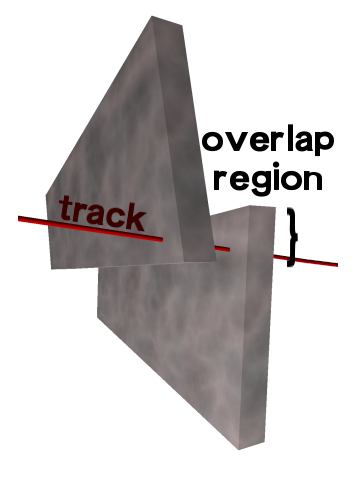
\includegraphics[width=0.3\linewidth]{overlaps.png} \hfill 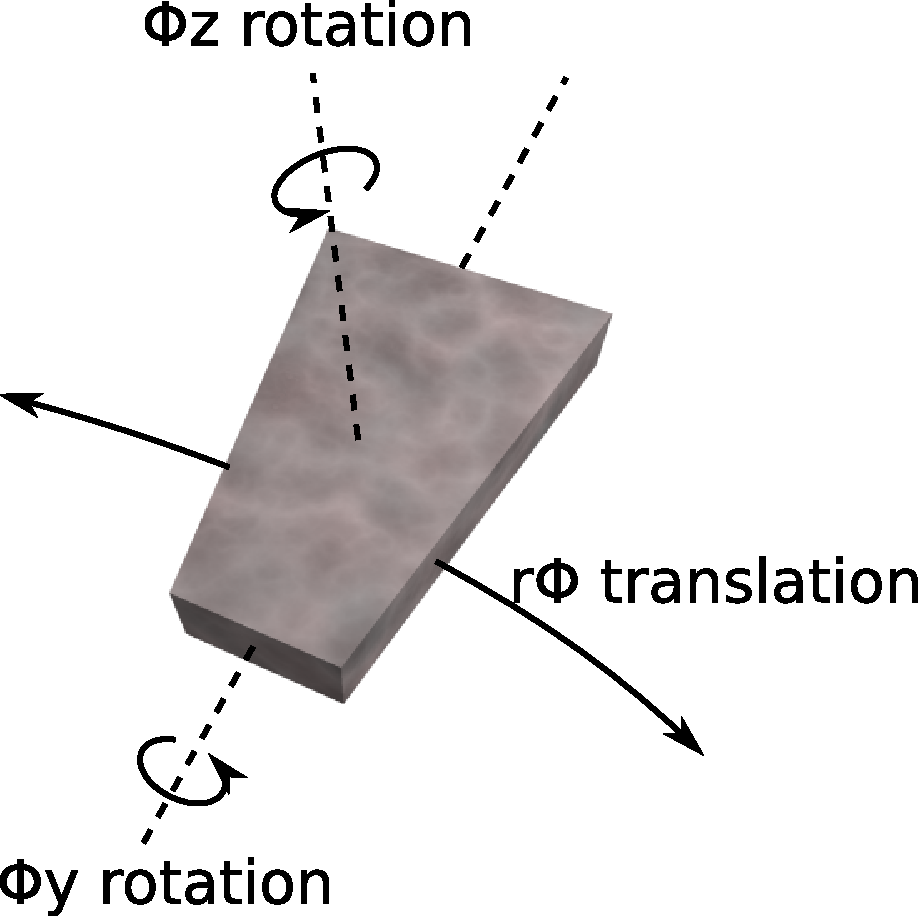
\includegraphics[width=0.4\linewidth]{csc_coordinates.pdf} \hfill \mbox{ }

\vspace{0.5 cm}
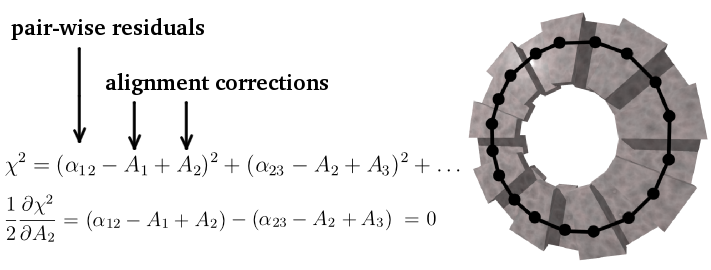
\includegraphics[width=\linewidth]{matrix_description_onestation.png}

\vspace{0.5 cm}
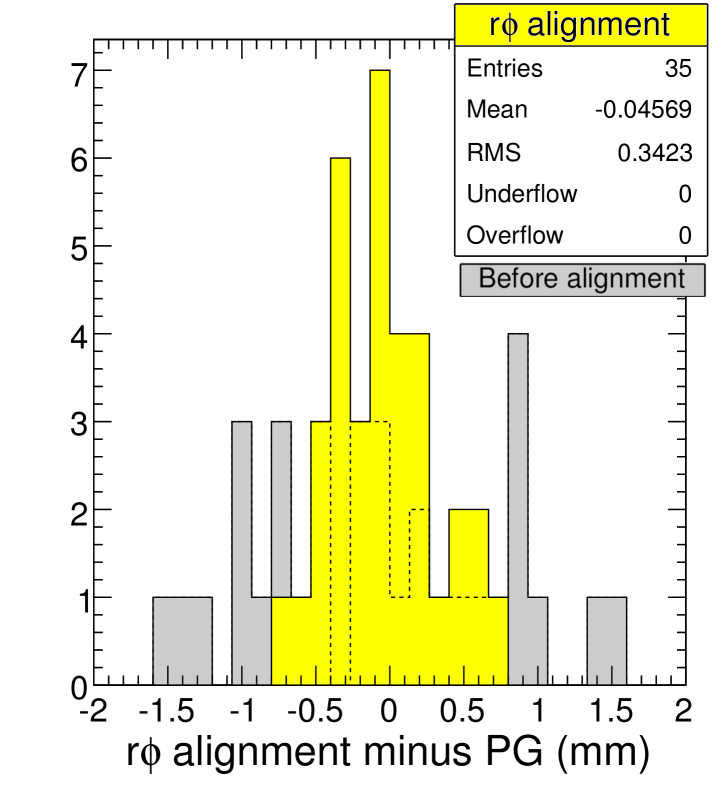
\includegraphics[width=0.5\linewidth]{data_rphi.png}
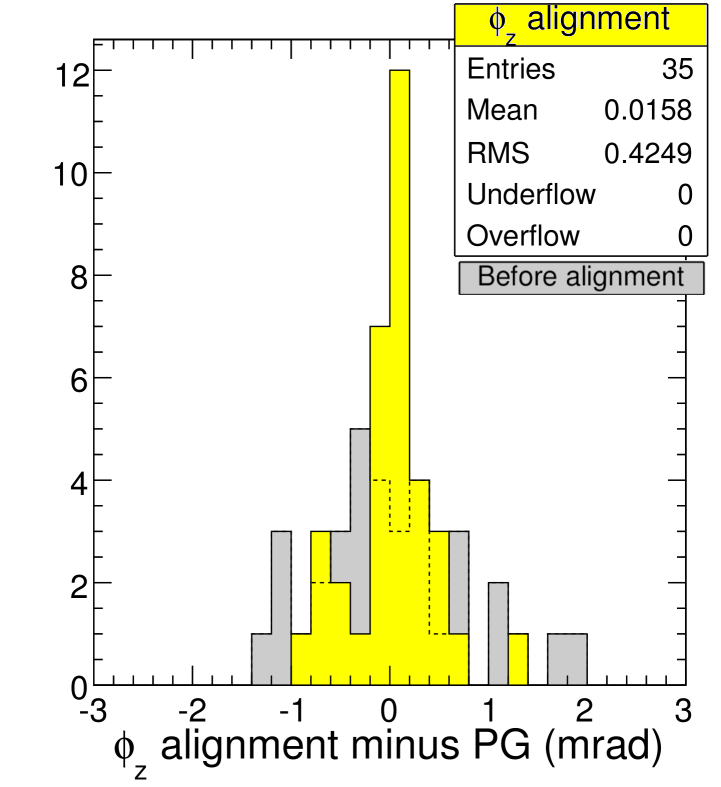
\includegraphics[width=0.5\linewidth]{data_phiz.png}
\end{columns}
\end{frame}

\begin{frame}
\frametitle{Why not upload the constants?}
\framesubtitle{Since beam-halo constants are good, why not use them in reconstruction?}

\begin{itemize}
\item Method requires complete rings
\begin{itemize}
\item only ME$-$2/1 and $-$3/1 were available: combination of high
  statistics due to being close to the beamline and status of chambers during those 9~minutes in 2008
\item to benefit from alignment, track would need to pass through exactly these two rings: very rare for CRAFT cosmic rays
\end{itemize}
\item Measurement performed with $\vec{B}=0$, unclear how much physical motion occured between beam-halo era and CRAFT
\end{itemize}

\vspace{0.5 cm}
\hspace{-0.83 cm} \textcolor{darkblue}{\Large And yet\ldots}

\vspace{0.1 cm}
\begin{itemize}
\item \textcolor{darkblue}{In a sense, we did:} one can think of the beam-halo/photogrammetry comparison as validating the {\it photogrammetry}
\item We uploaded all of the CSC photogrammetry chamber positions: they are being used in reconstruction now
\end{itemize}
\end{frame}

\begin{frame}
\frametitle{Completeness of rings (1/2)}

\begin{itemize}
\item Most rings are reliably complete, thanks to 6 months of work
\item Snapshot from June 11 (99322):
\end{itemize}

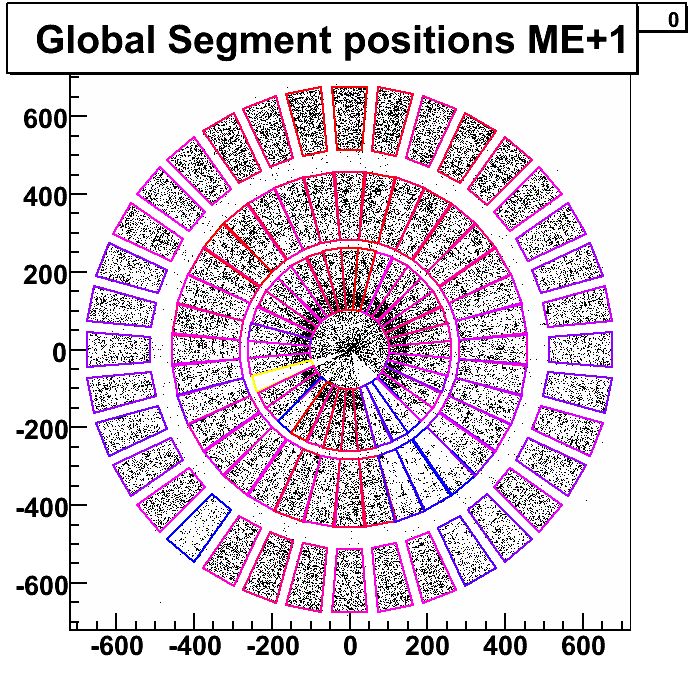
\includegraphics[width=0.25\linewidth]{cscpopulation_p1.png}
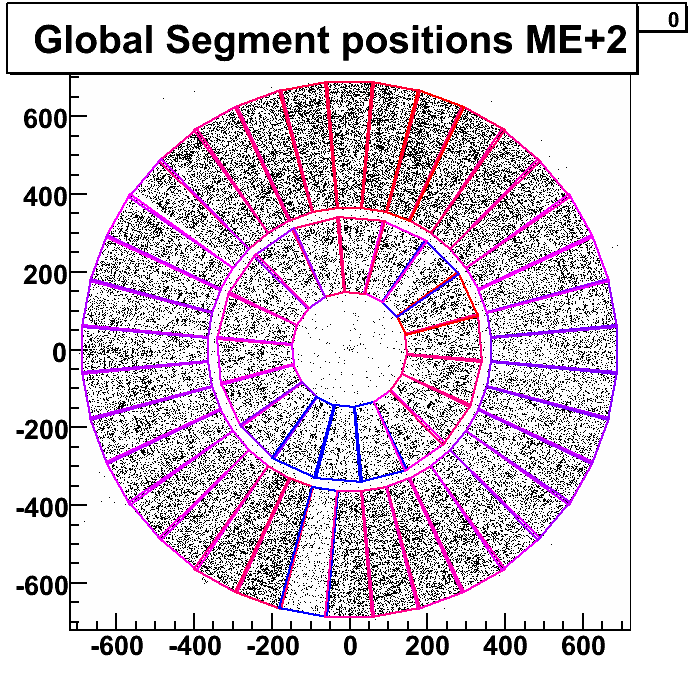
\includegraphics[width=0.25\linewidth]{cscpopulation_p2.png}
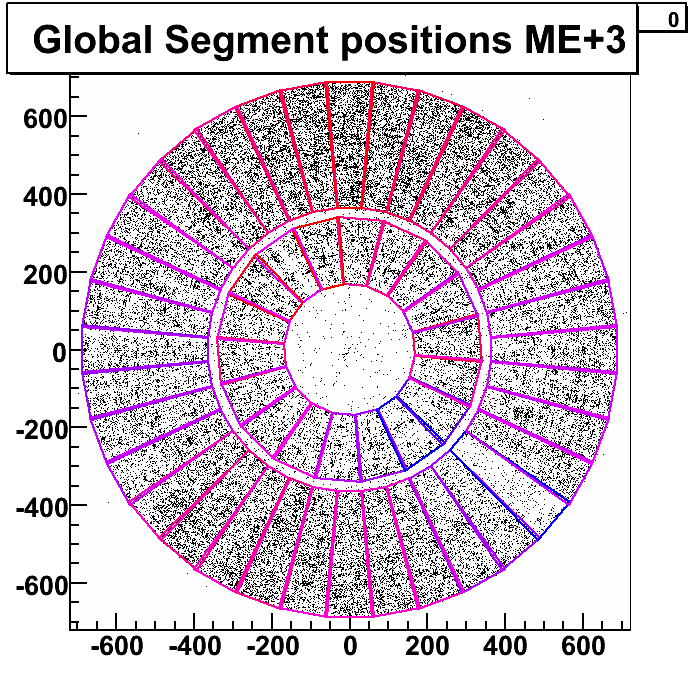
\includegraphics[width=0.25\linewidth]{cscpopulation_p3.png}
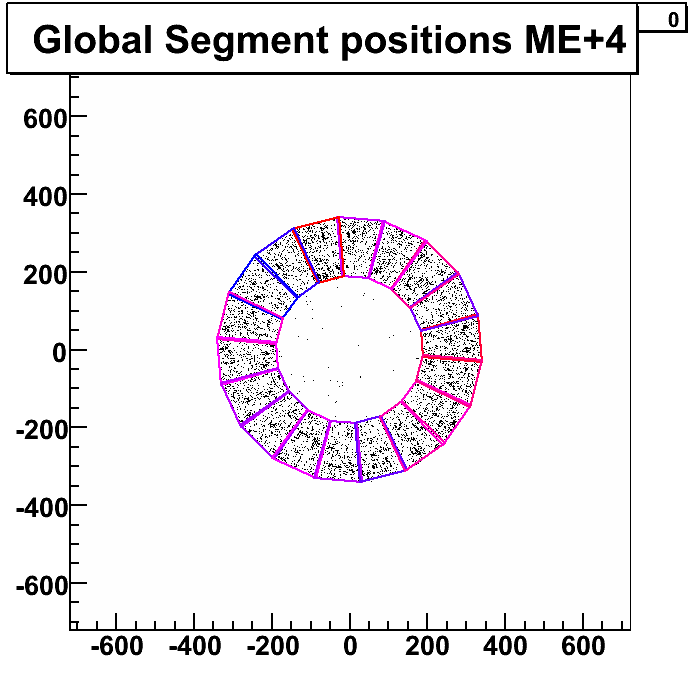
\includegraphics[width=0.25\linewidth]{cscpopulation_p4.png}

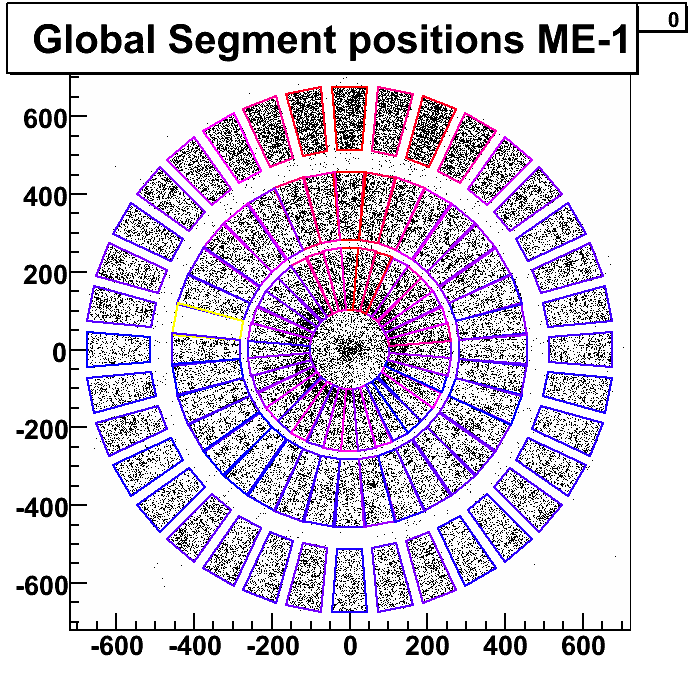
\includegraphics[width=0.25\linewidth]{cscpopulation_m1.png}
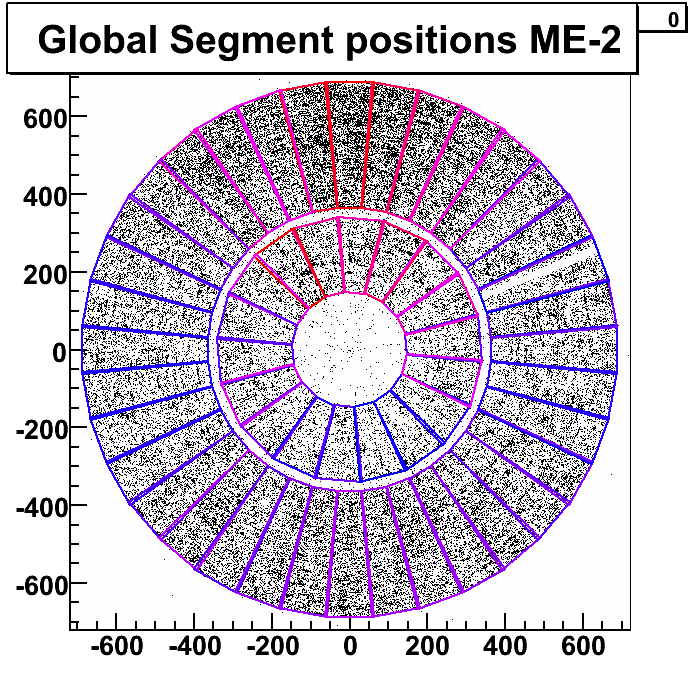
\includegraphics[width=0.25\linewidth]{cscpopulation_m2.png}
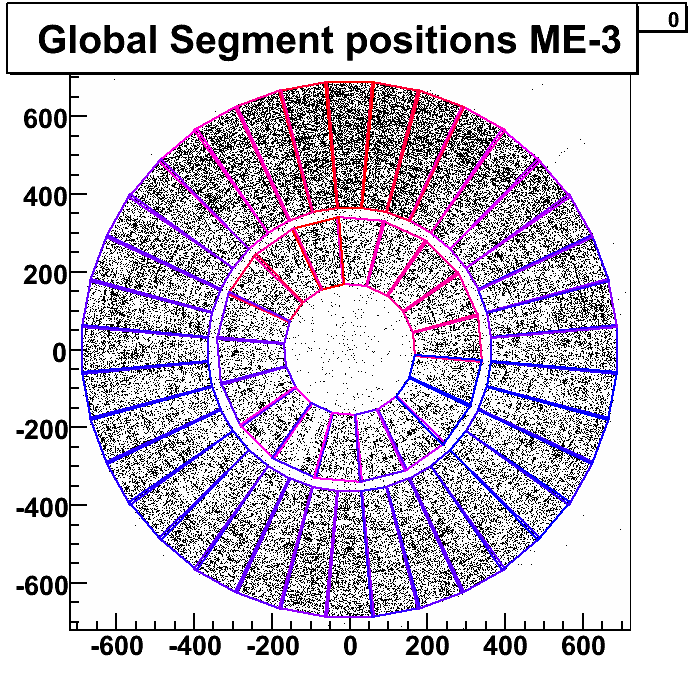
\includegraphics[width=0.25\linewidth]{cscpopulation_m3.png}
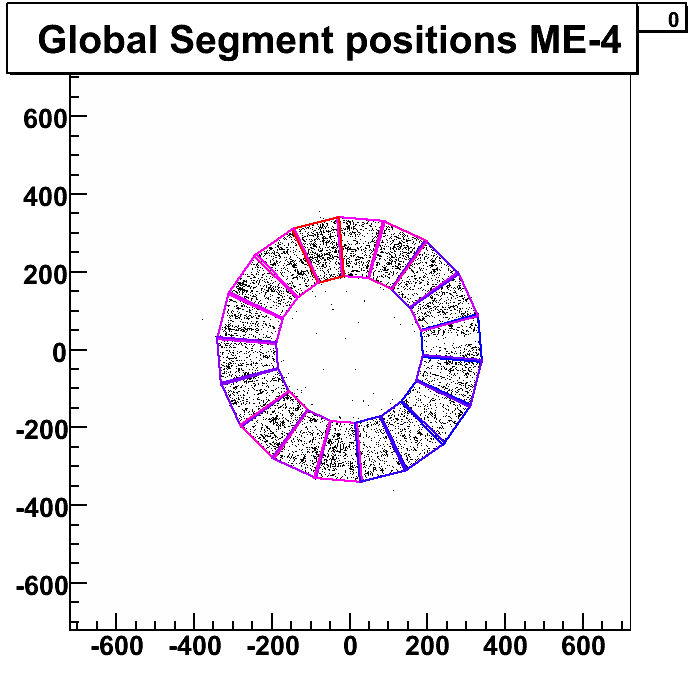
\includegraphics[width=0.25\linewidth]{cscpopulation_m4.png}

\hfill \scriptsize A.~Kubik
\end{frame}

\begin{frame}
\frametitle{Completeness of rings (2/2)}

\vspace{0.5 cm}
\begin{columns}
\column{0.5\linewidth}
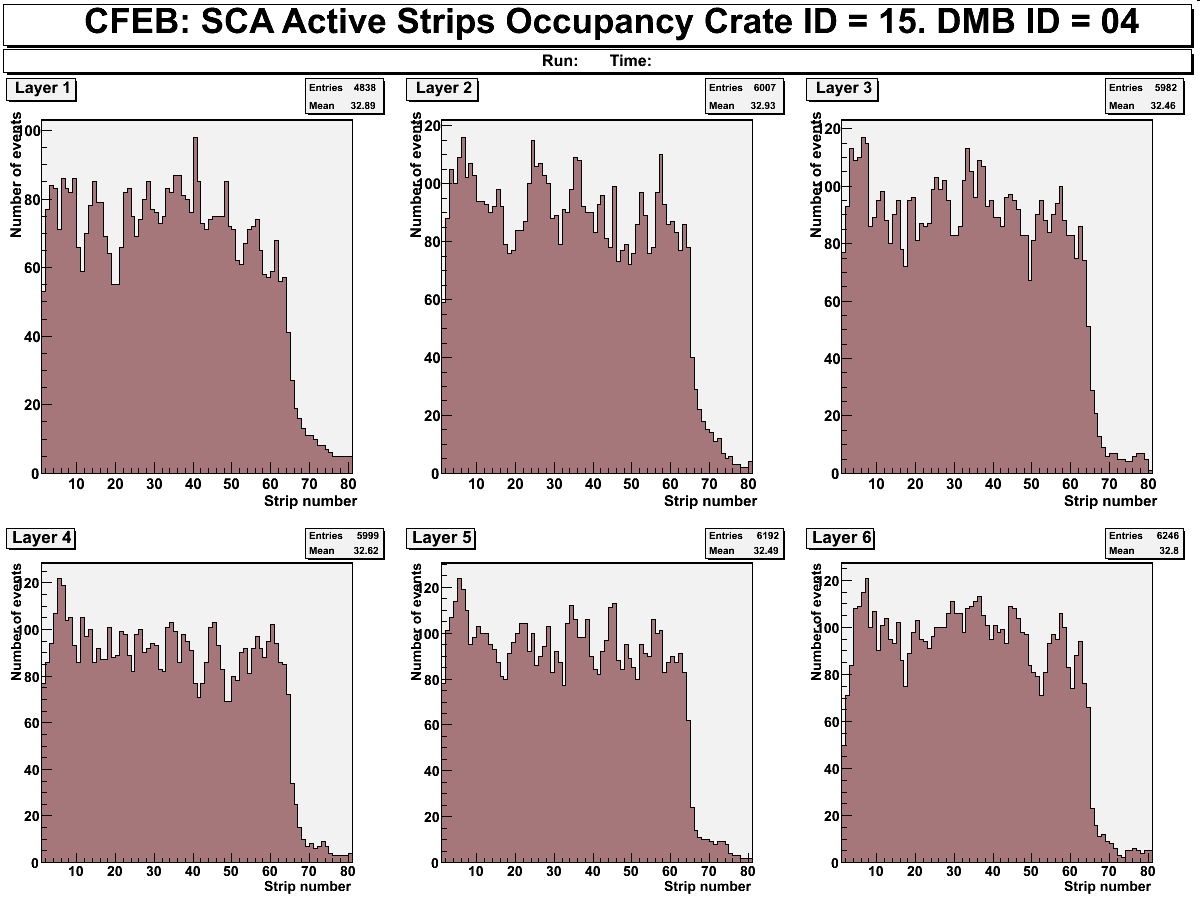
\includegraphics[width=\linewidth]{armando_CFEB5.png}

\column{0.5\linewidth}
\begin{itemize}
\item Something to be careful about: CFEB inefficiencies
\begin{itemize}
\item since overlaps procedure only requires hits along the edges of CSCs, this is only a problem when first or last CFEB (1 or 5) is inefficient/dead
\end{itemize}
\end{itemize}
\end{columns}

\vspace{0.2 cm}
\begin{itemize}
\item Armando's list of bad CFEBs includes 3 bad edge CFEBs, all in different rings {\scriptsize ($+$1/2/15.1, $+$2/2/15.5, $+$3/2/19.5)}
\item Overlaps procedure can be modified to fill-in missing information by assuming perfect closure (sum of residuals around ring = 0)
\item This is different from a dead chamber, which would remove two overlaps measurements, one from each side
\end{itemize}
\end{frame}

\section*{2. Baseline procedure}
\begin{frame}
\begin{center}
\Huge \textcolor{blue}{2. Baseline procedure (tracker-to-muon chambers)}
\end{center}
\end{frame}

\begin{frame}
\frametitle{2. Baseline procedure}
\begin{itemize}\setlength{\itemsep}{0.15 cm}
\item \textcolor{darkblue}{Method:} {\scriptsize (1)} fit track in tracker, {\scriptsize (2)} propagate it to muon chamber, \\ {\scriptsize (3)} align chamber to agree with track
\item In the long run ($\gtrsim 50$~pb$^{-1}$), all chambers can be aligned like this
\item Cosmic rays illuminate many DT chambers (wheels $-$1, 0, $+$1, except stations 1 and 7)
\item Aligning the barrel in CRAFT improved our understanding about the following:
\begin{itemize}
\item how can we disentangle alignment from magnetic field effects when we propagate tracks from the tracker? {\scriptsize (resolved)}
\item how can we be sure that the tracker is not globally distorted? {\scriptsize (we have some techniques, but not completely resolved)}
\item also developed much more robust fitting procedures, less sensitive to single-scattering tails
\end{itemize}
\item These are the ``non-local'' issues, complimentary to what we learned with beam-halo; most carries over from DT to CSC
\end{itemize}
\end{frame}

\begin{frame}
\frametitle{Magnetic field effects}

\begin{columns}
\column{0.5\linewidth}
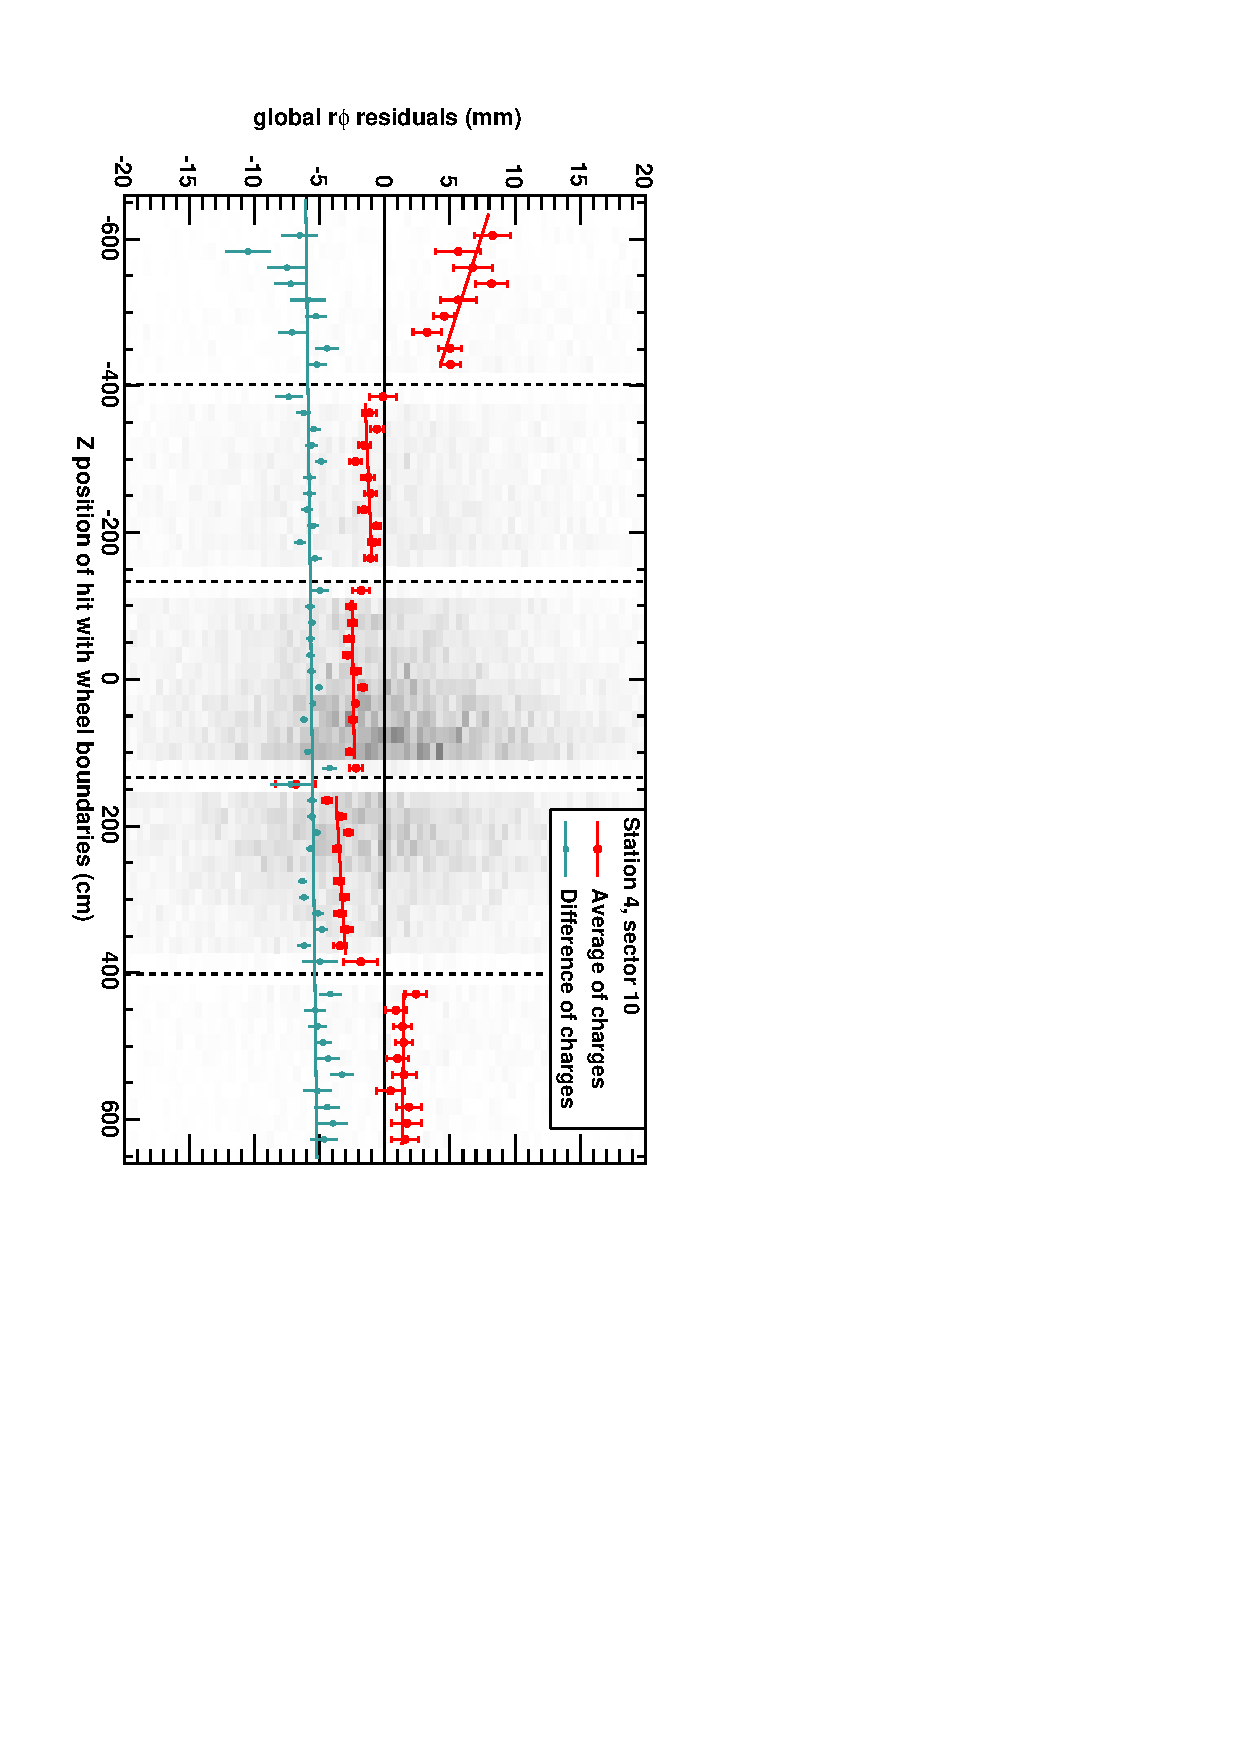
\includegraphics[height=\linewidth, angle=90]{demo_of_bfield.pdf}

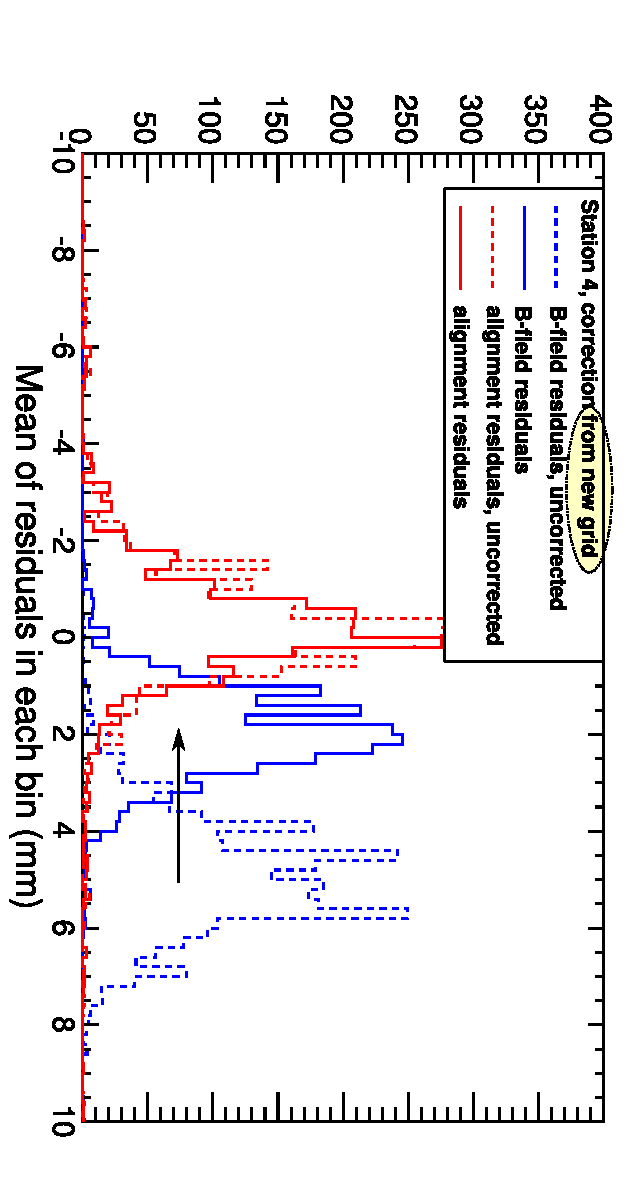
\includegraphics[height=\linewidth, angle=90]{newgrid_corrections_station4.pdf}

\begin{columns}
\column{0.4\linewidth}
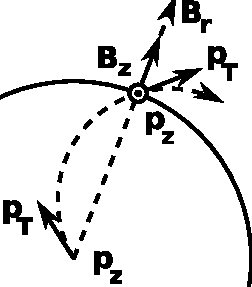
\includegraphics[width=\linewidth]{bfield_components.pdf}
\column{0.6\linewidth}
\scriptsize $\vec{B_z} \cdot \vec{p_T}$ and $\vec{B_r} \cdot \vec{p_z}$ both cause $r\phi$ residuals that are antisymmetric in charge
\end{columns}

\column{0.5\linewidth}
\begin{itemize}
\item Residuals have seperable components when viewed as a function of charge
\begin{itemize}
\item alignment is independent of the tracks' charge
\item $\vec{B}$ (and $dE/dx$) errors are antisymmetric in charge
\end{itemize}

\item \textcolor{red}{Alignment residuals (red)} have discontinuities at chamber boundaries before alignment and are unaffected by changing the $\vec{B}(\vec{x})$ map

\item \textcolor{blue}{Charge antisymmetric residuals (blue)} are insensitive to chamber geometry and change dramatically with new maps
{\scriptsize (example from February)}

\end{itemize}
\end{columns}
\end{frame}

\begin{frame}
\frametitle{Track-source distortion}
\begin{itemize}\setlength{\itemsep}{0.1 cm}
\item Alignment information is propagated from the tracker: if the tracker is misaligned, the muon system will be too
\item Two classes of distortions:

\vspace{-0.3 cm}
\begin{columns}
\column{0.44\linewidth}
\begin{itemize}
\item \textcolor{darkblue}{small-scale:} all collisions muons for a chamber point back to the same misaligned region of the tracker {\scriptsize (right, from CSA08)}
\end{itemize}
\column{0.4\linewidth}
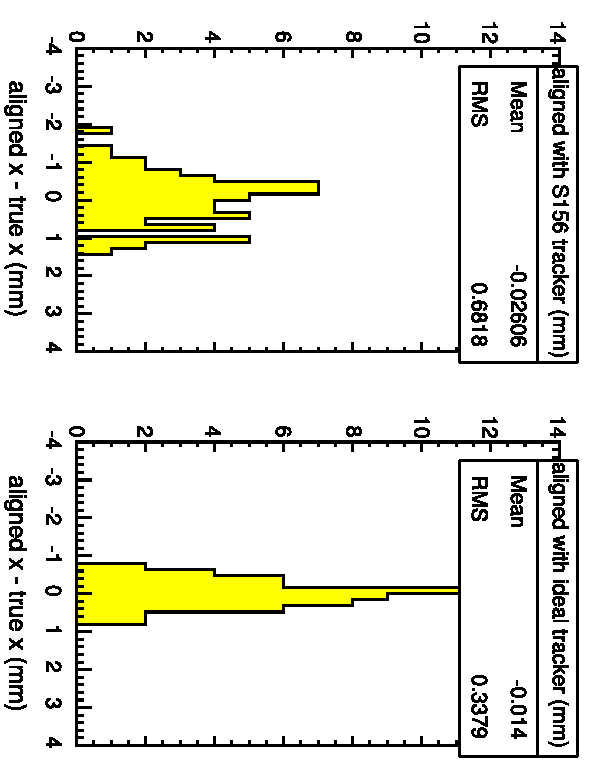
\includegraphics[height=\linewidth, angle=90]{muonalignment_MB1_dep_on_tracker.pdf}
\end{columns}

\mbox{\hspace{-0.32 cm}\begin{minipage}{1.1\linewidth}
\begin{itemize}
\item \textcolor{darkblue}{global:} tracker weak mode gets imprinted onto the muon system, something $\propto$ $\sin\phi$, $\sin 2\phi$, $z$, $z^2$, etc., or combinations
\end{itemize}
\end{minipage}}

\item Muon alignment is much less sensitive to errors in track
  direction \\ ($\phi$ and $\eta$) than errors in track curvature ($p_T$)
\begin{itemize}
\item curvature errors grow quadratically as track propagates
\end{itemize}

\item In cosmic ray alignments, \textcolor{darkblue}{small-scale} distortions are ``washed out'' by the fact that cosmics don't all point to the same spot
\end{itemize}
\end{frame}

\begin{frame}
\frametitle{Observed global distortion}
\begin{columns}
\column{0.5\linewidth}
\begin{itemize}
\item $20 < p_T < 100$~GeV tracks and $100 < p_T < 200$~GeV tracks yield different alignments, with a different overall shape {\scriptsize (right)}
\begin{itemize}
\item rotation and twist of the barrel {\it that depends on $p_T$}
\end{itemize}
\end{itemize}

\column{0.5\linewidth}
\mbox{ }

{\tiny \hfill Differences in chamber $\phi$ positions between alignments}

\vspace{0.1 cm}
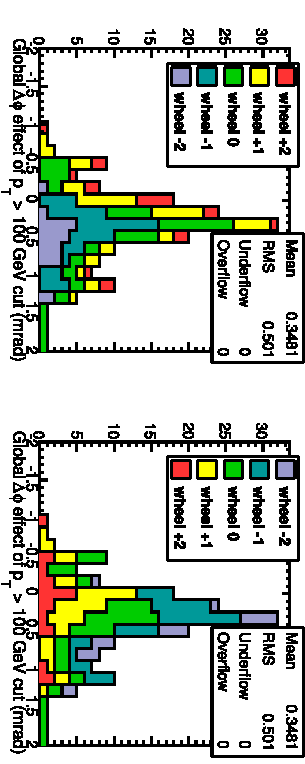
\includegraphics[height=\linewidth, angle=90]{data_effect_of_100GeVcut3.pdf}

\vspace{-0.15 cm}
{\tiny \mbox{ } \hfill same chambers, opposite stacking order \hfill \mbox{ }}

\vspace{-0.3 cm}
\end{columns}

\vspace{0.2 cm}
\mbox{\hspace{-0.32 cm}\begin{minipage}{\linewidth}
\begin{itemize}
\item Magnetic field/material corrections have been applied--- this effect in residuals is independent of charge, not a $\vec{B}$, $dE/dx$ issue \mbox{\scriptsize (bottom-left)\hspace{-1 cm}}
\end{itemize}
\end{minipage}}

\begin{columns}
\column{0.35\linewidth}
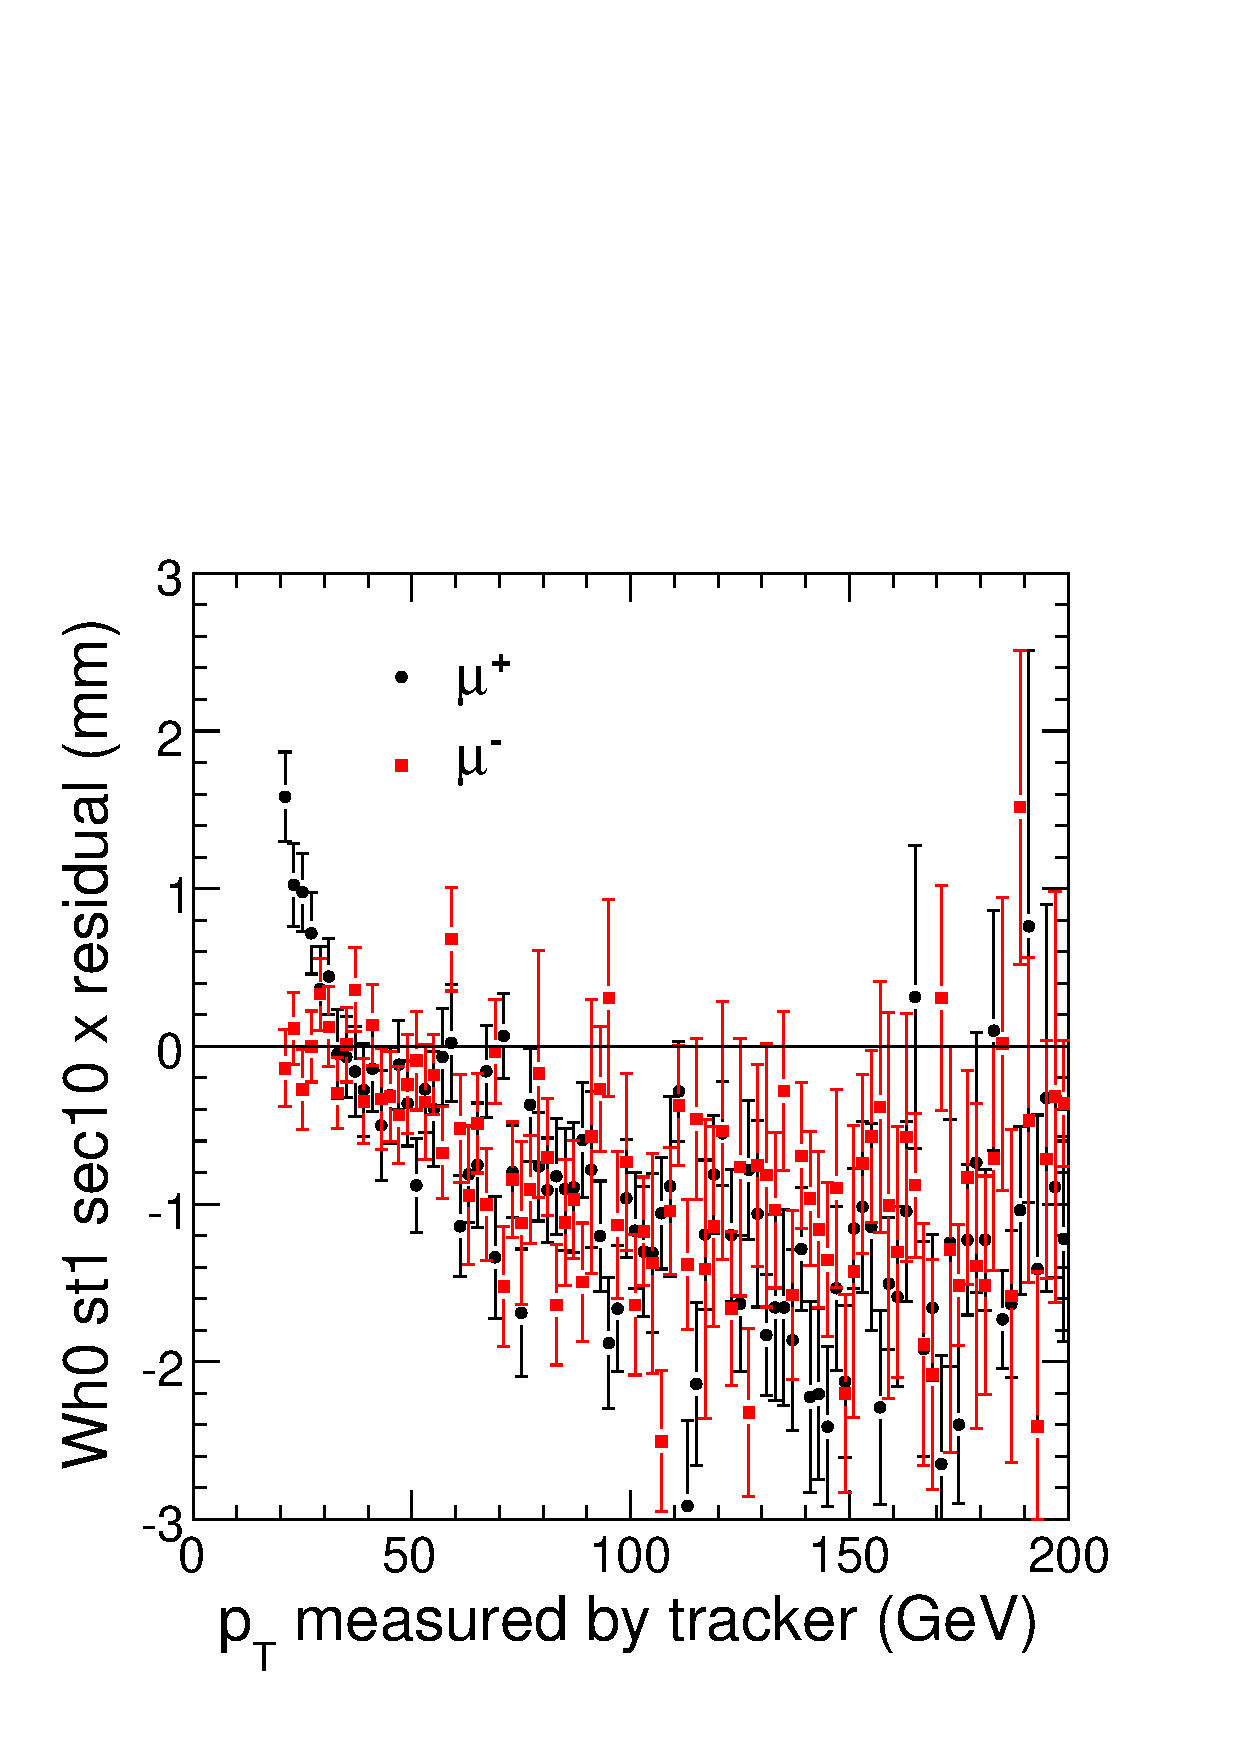
\includegraphics[width=\linewidth]{resid_vs_pt.pdf}

\column{0.65\linewidth}
\begin{itemize}
\item High-$p_T$ alignment yields more consistent momentum measurements at all momenta
\end{itemize}

\hfill 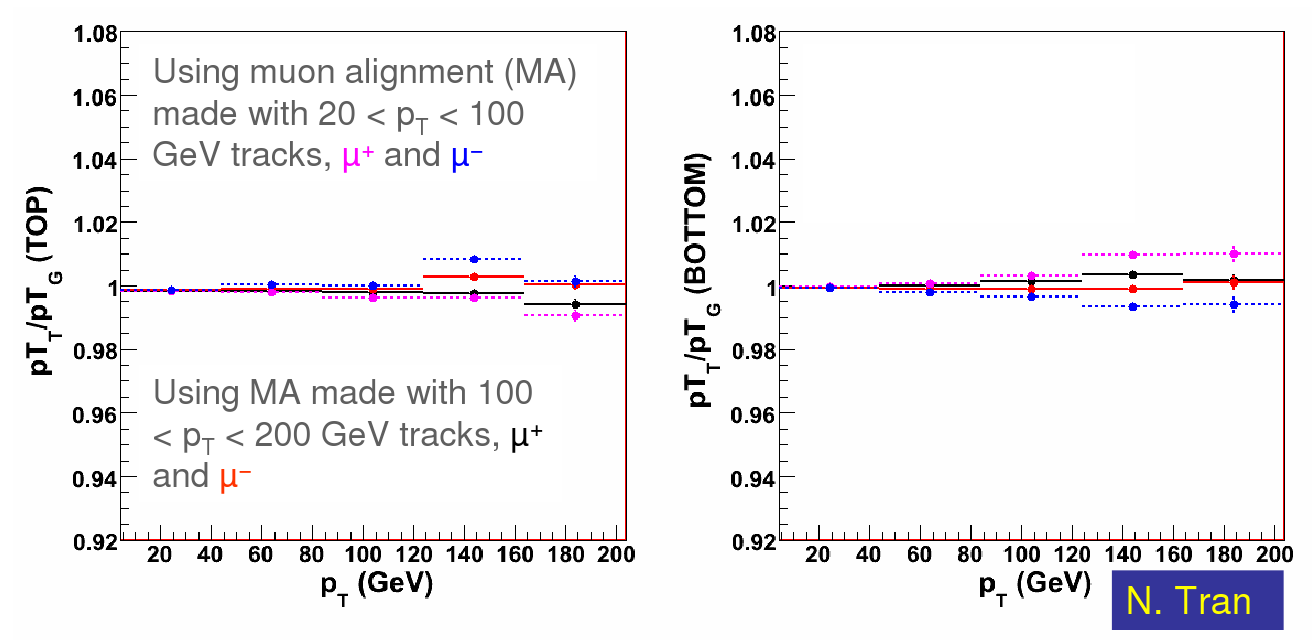
\includegraphics[width=0.9\linewidth]{cosmicsplitting_nhan.png}
\end{columns}
\end{frame}

\begin{frame}
\frametitle{Tracker curl {\it hypothesis}}
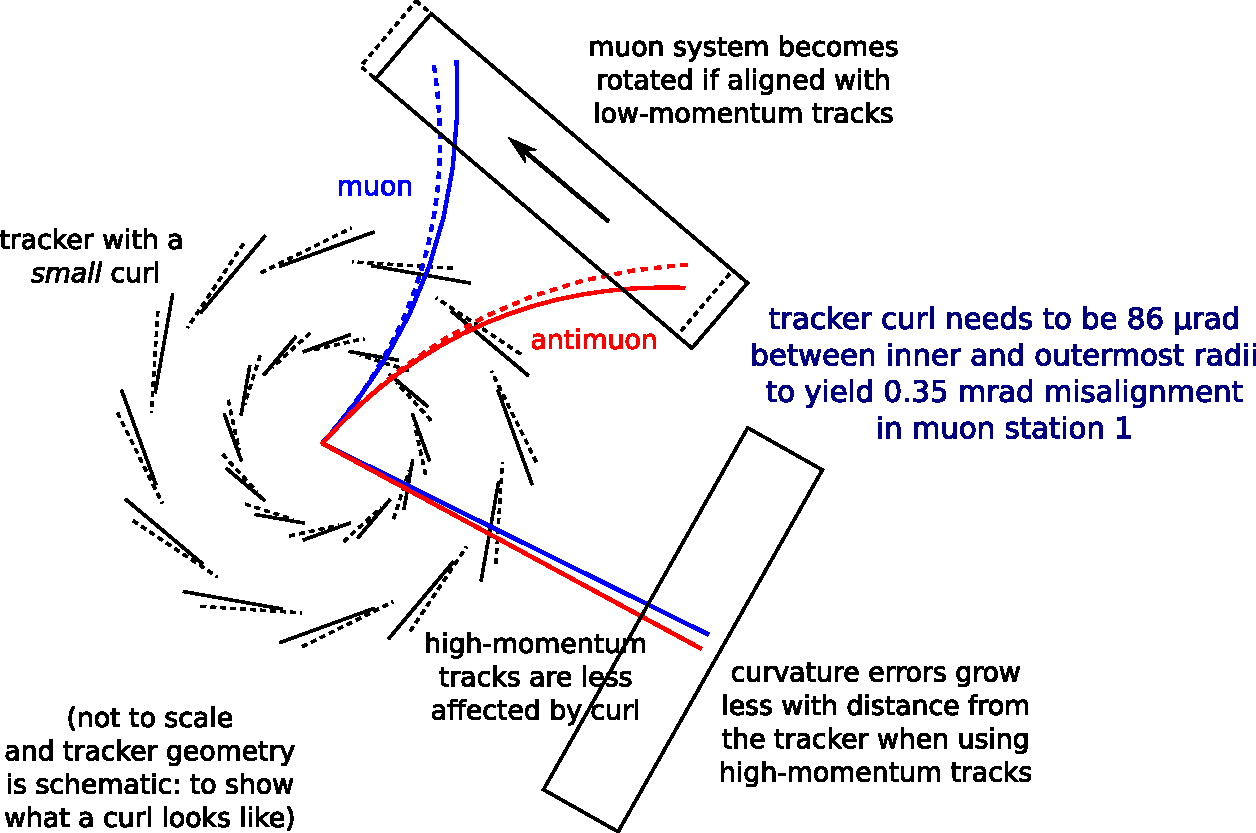
\includegraphics[width=\linewidth]{curl_explanation.pdf}
\end{frame}

\begin{frame}
\frametitle{Tracker curl {\it constraints}}

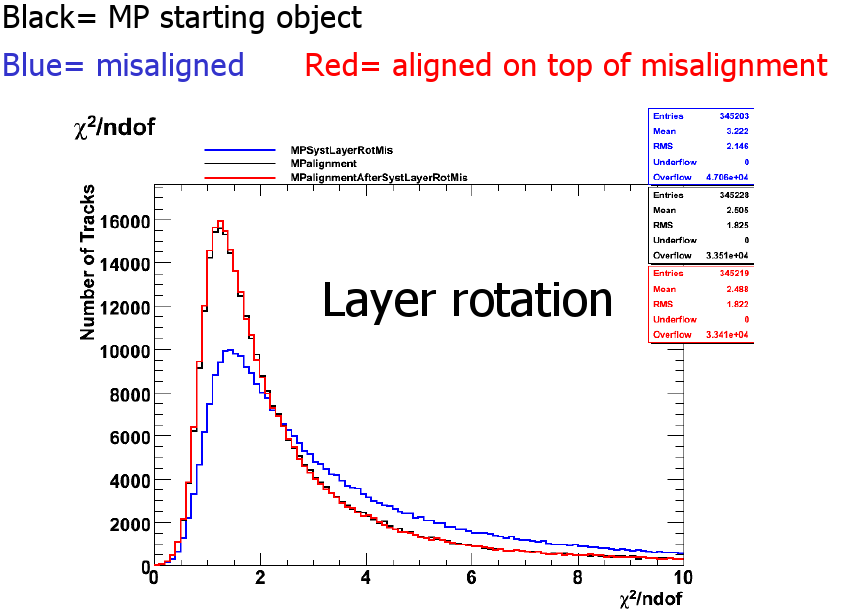
\includegraphics[width=0.55\linewidth]{tracks_are_sensitive_to_curl.png} \hfill 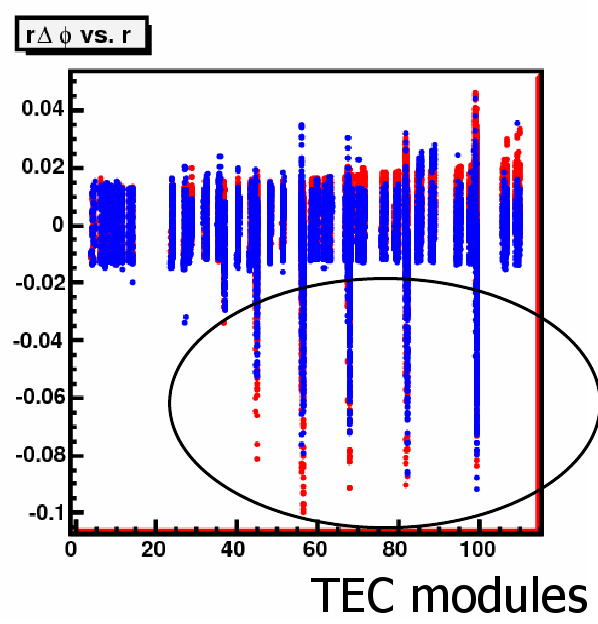
\includegraphics[width=0.35\linewidth]{curl_is_not_86microns.png}

\begin{itemize}
\item Studies performed in CRAFT data \hfill \textcolor{darkblue}{\scriptsize Zijin Guo, Roberto Castello}
\item \textcolor{darkblue}{Left:} tracker tracks are sensitive to 300~$\mu$rad curl (\textcolor{blue}{blue:\ adding curl worsens $\chi^2$} and \textcolor{red}{red:\ re-aligning restores it})
\item \textcolor{darkblue}{Right:} also restores wafer positions within 150~$\mu$rad \mbox{except TEC\hspace{-1 cm}}
\begin{itemize}
\item TEC not used in muon alignment; not relevant here
\item restored chamber positions randomly distributed around zero: \textcolor{darkblue}{no {\it systematic} trend on the scale of 86~$\mu$rad}
\end{itemize}
\item Source of distortion has not been explained: ongoing work\ldots
\end{itemize}
\end{frame}

\begin{frame}
\frametitle{Redundant binning}
\begin{itemize}
\item To partially distinguish track biases from real misalignments,
  plot residuals in finer bins than the chamber size
\begin{itemize}
\item global chamber distortions and propagation errors have a smooth
  effect on residuals
\item misalignments introduce sharp discontinuities at the chamber
  boundaries (dotted lines) because they are large rigid bodies
\end{itemize}

{(I'll use this again later in the talk, for the endcap)}
\end{itemize}
\begin{center}
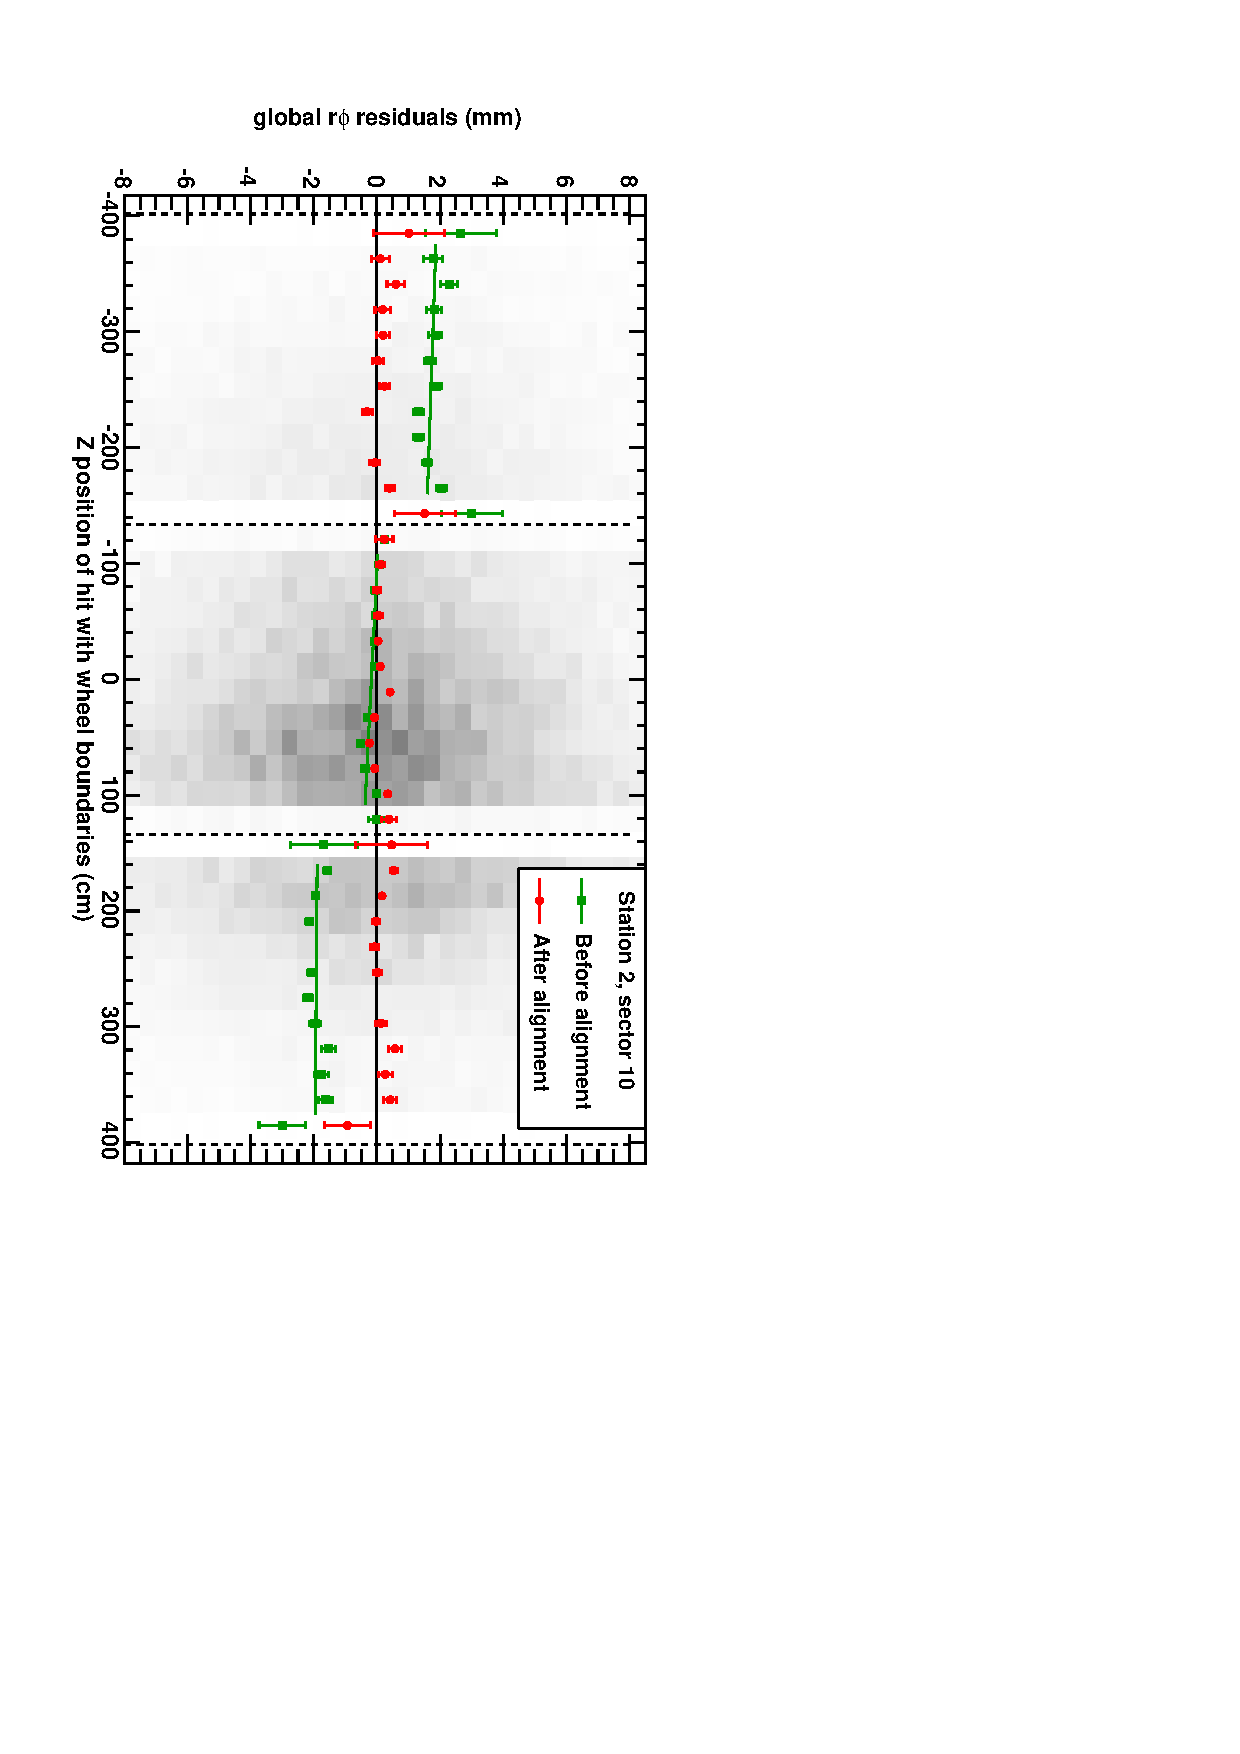
\includegraphics[height=0.75\linewidth, angle=90]{example_mapplot4.pdf}
\end{center}
\end{frame}

\begin{frame}
\frametitle{Extra constraint in the endcap}

\begin{itemize}
\item In the endcap, we can run the Baseline and Overlaps procedures with the same tracks
\item Orthogonal sets of connectors (relative alignments):
\begin{itemize}
\item chamber positions measured relative to tracker with Baseline
\item relative to next-door ring neighbors from Overlaps
\item should observe nothing more than whole-ring misalignment
\end{itemize}
\item Sensitive to elliptical distortions of the tracker or endcap track-propagation
\end{itemize}

\vspace{-0.5 cm}
\begin{center}
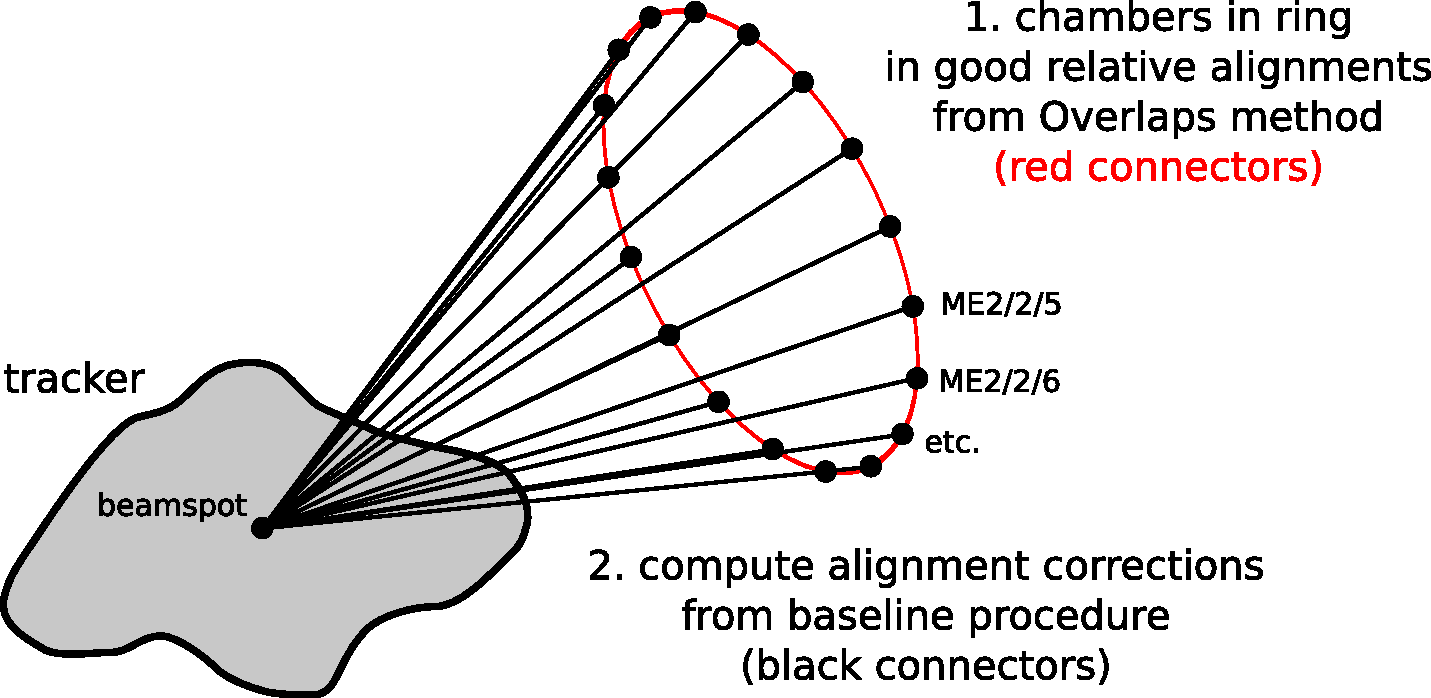
\includegraphics[width=0.8\linewidth]{baseline_overlaps_interference.pdf}
\end{center}
\end{frame}

\begin{frame}
\frametitle{Improved alignment fits}

\begin{itemize}
\item Based on CRAFT experience, we revised our fit model in two ways:
\begin{itemize}
\item expanded residuals to include angular components, to improve
  resolution on angular alignments
\item one many-parameter fit for alignment and \mbox{instrumental effects\hspace{-1 cm}}
\end{itemize}
\end{itemize}

\begin{columns}
\column{0.5\linewidth}
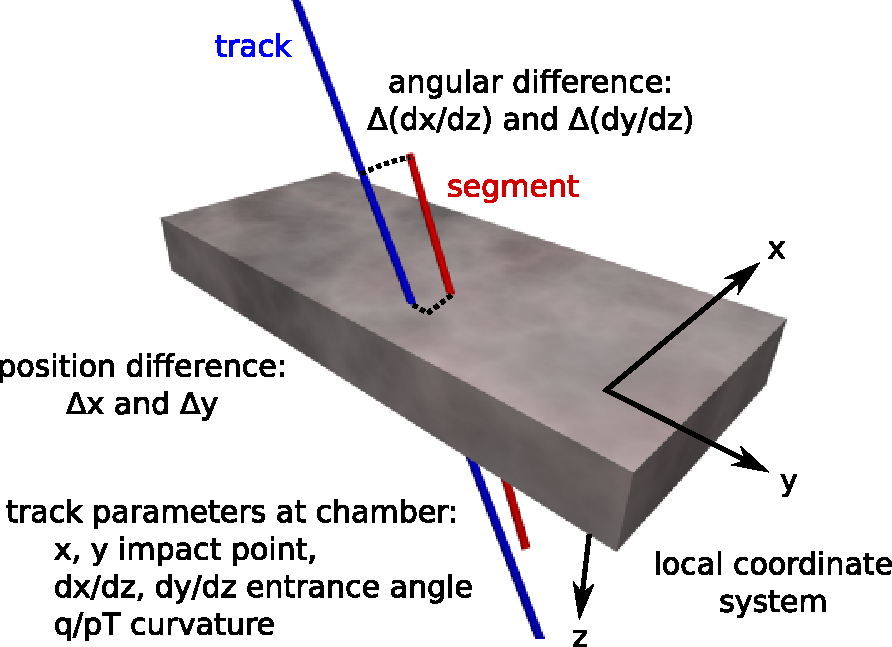
\includegraphics[width=\linewidth]{dt_coordinates.pdf}

\column{0.5\linewidth}
\begin{itemize}
\item \mbox{DT chamber measures 2-D\hspace{-1 cm}} \\ position and direction: 4-component residuals
\item Access to 6 rigid-body alignment parameters \mbox{(3~translation, 3~rotation)\hspace{-0.5 cm}} \\ through a $6\times 4$ matrix \\ instead of \mbox{the usual $6\times 2$\hspace{-1 cm}}
\end{itemize}
\end{columns}

\vspace{0.3 cm}
\begin{itemize}
\item CSC wire groups are too granular for alignment: \mbox{$\mathcal{O}(\mbox{cm})$ non-Gaussian\hspace{-1 cm}}
\item Strips measure 1-D position and direction: 2-component residuals
\item Access to 6-DOF through a $6\times 2$ matrix (instead of $6\times 1$), \\ though in practice only 3 DOF can be resolved with precision
\end{itemize}
\end{frame}

\begin{frame}
\frametitle{Sample fit results: \only<1>{DT MC}\only<2>{DT data}\only<3>{CSC MC}}

\vspace{0.25 cm}
\begin{columns}
\column{0.5\linewidth}

\mbox{ } \hfill \textcolor{darkblue}{Before alignment} \hfill \mbox{ }

\only<1>{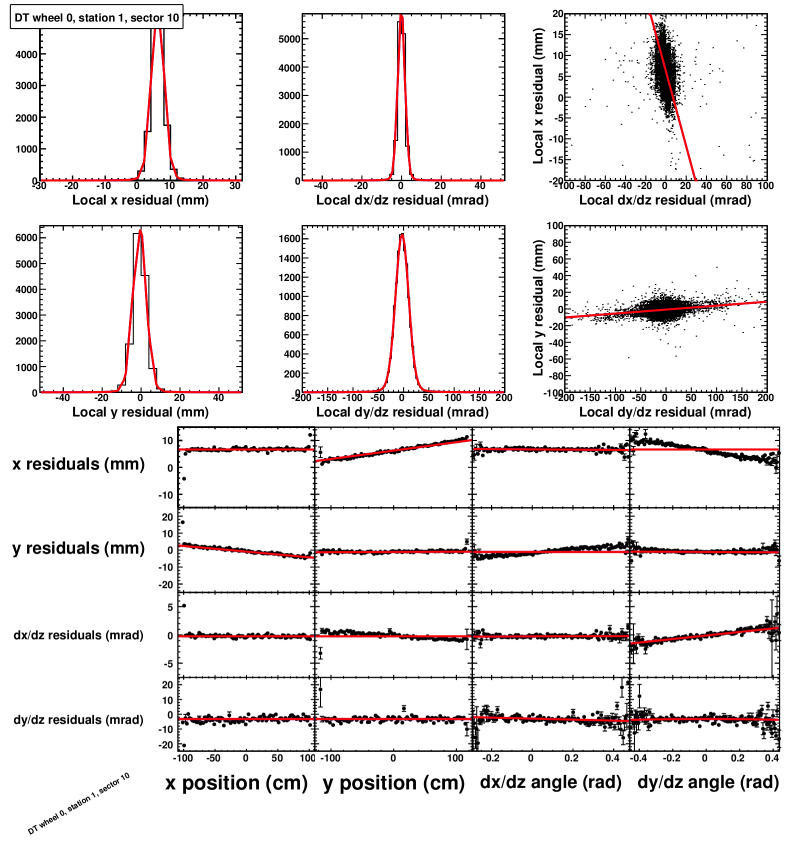
\includegraphics[width=\linewidth]{exampleMC_wh0st1sec10_before.png}}\only<2>{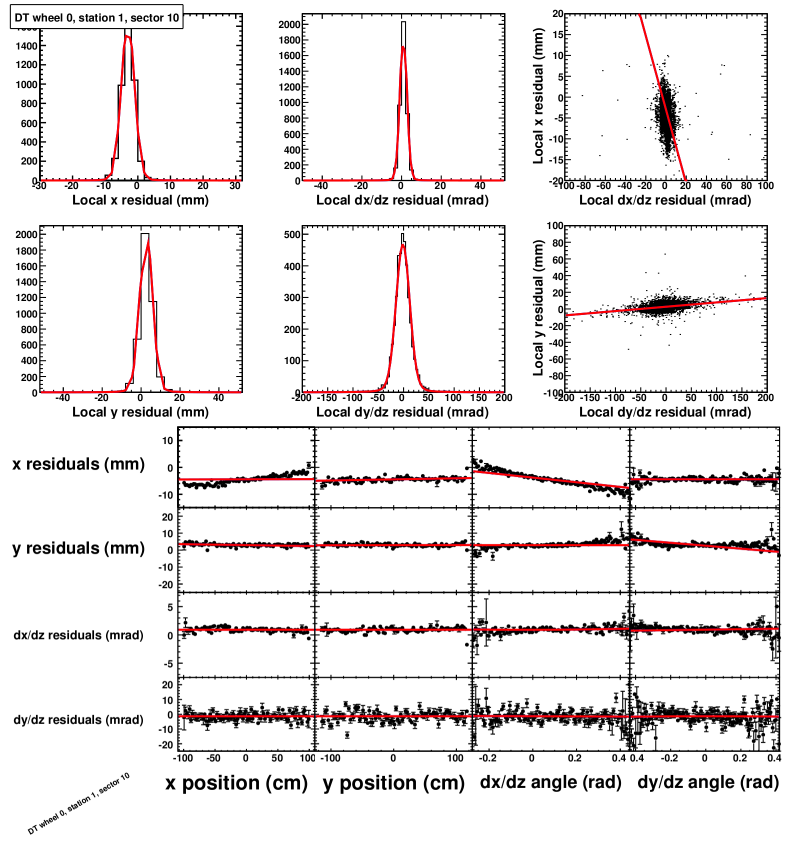
\includegraphics[width=\linewidth]{exampleData_wh0st1sec10_before.png}}\only<3>{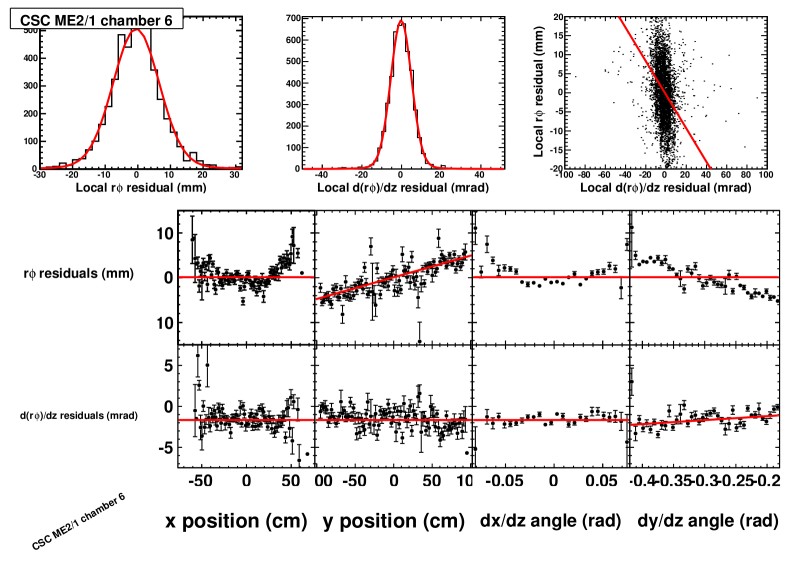
\includegraphics[width=\linewidth]{mcfit_cscexample_before.png}}

\column{0.5\linewidth}

\mbox{ } \hfill \textcolor{darkblue}{After alignment} \hfill \mbox{ }

\only<1>{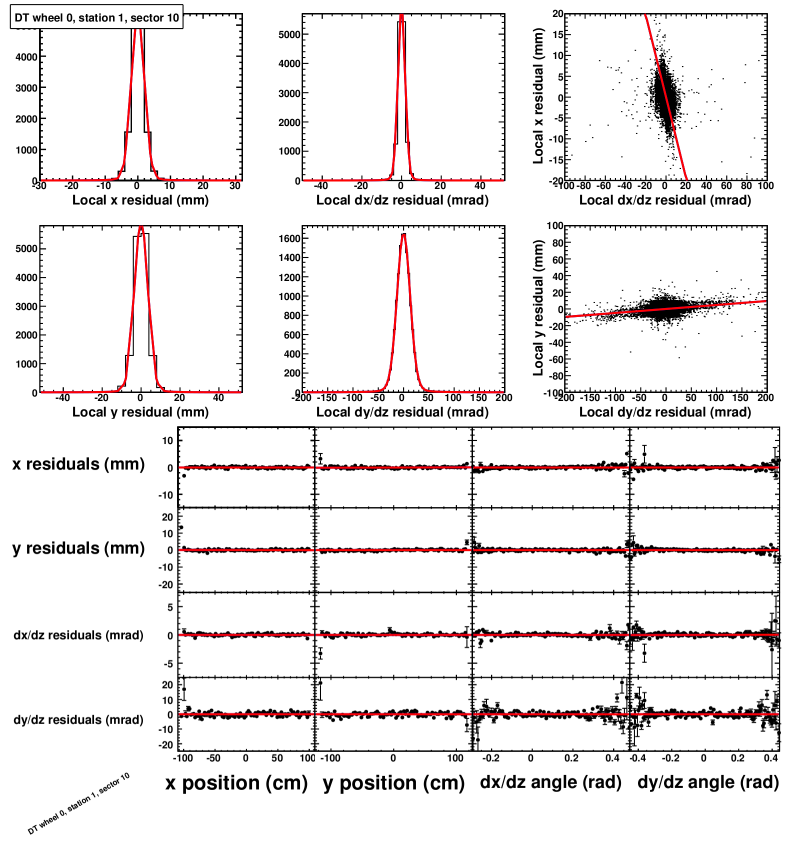
\includegraphics[width=\linewidth]{exampleMC_wh0st1sec10_after.png}}\only<2>{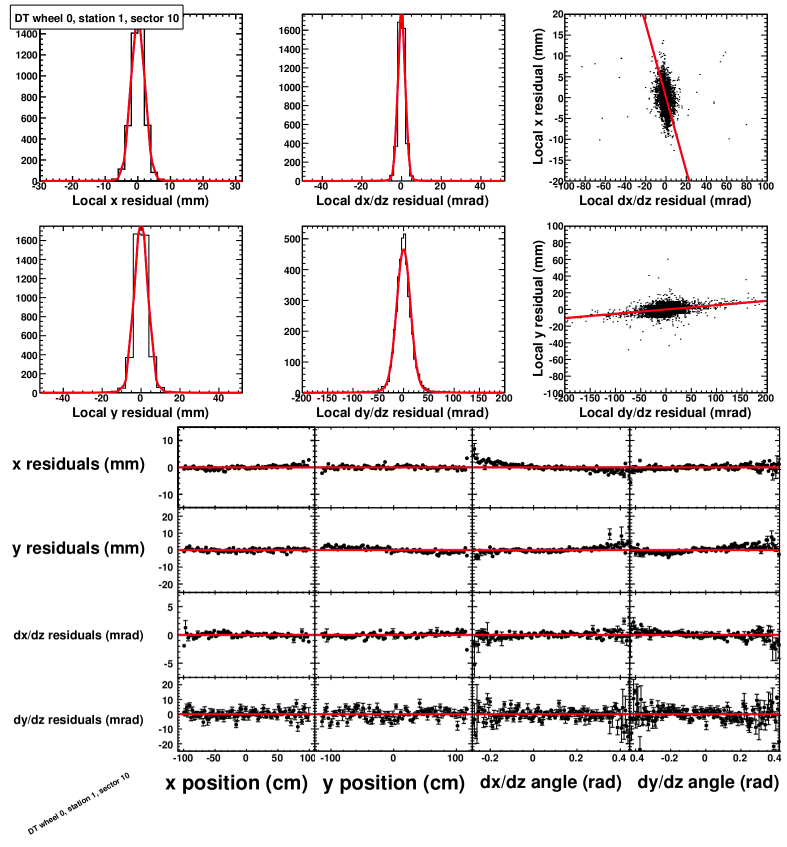
\includegraphics[width=\linewidth]{exampleData_wh0st1sec10_after.png}}\only<3>{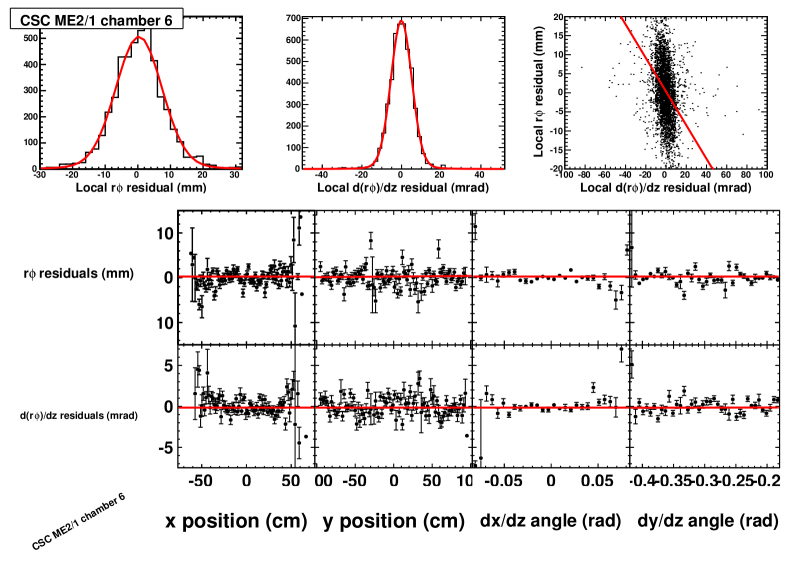
\includegraphics[width=\linewidth]{mcfit_cscexample_after.png}}

\end{columns}

\begin{itemize}
\item Projection of \textcolor{red}{fits (all parameters = 0 other than the one shown)} overlaid on \only<1>{{\it simulated} cosmic rays}\only<2>{{\it real} CRAFT data}\only<3>{simulated {\it collisions}} (profile plots) \only<1>{for one chamber}\only<2>{for the same chamber}
\item \only<1>{Method works well in Monte Carlo}\only<2>{Largely the same behavior in data; studying small discrepancies}\only<3>{Given the level of DT agreement, we don't expect show-stoppers}
\end{itemize}
\end{frame}

\begin{frame}
\frametitle{Why only 3 parameters?}

\begin{itemize}
\item Only the \textcolor{red}{red terms} are significant; the rest are small because
\begin{itemize}\setlength{\itemsep}{0.1 cm}
\item $\frac{dx}{dz}$ is the non-radial, non-longitudinal component of track direction: only very low $p_T$ tracks would have non-negligible $\frac{dx}{dz}$
\item $R$ is the distance from the hit to the beamline, large compared to $x$ coordinates in the chamber
\end{itemize}
\end{itemize}

\vspace{-0.5 cm}
{\scriptsize \begin{eqnarray*}
\mbox{\small (residuals)} & \mbox{\hspace{-0.3 cm}} = \mbox{\hspace{-0.3 cm}} & \mbox{\small (matrix)} \cdot \mbox{\small (alignment parameters)} \\
\renewcommand{\arraystretch}{3}
\left(\begin{array}{c}
{\Delta r\phi} \\
{\Delta \dfrac{dr\phi}{dz}} \\
\end{array}\right)
& \mbox{\hspace{-0.3 cm}} = \mbox{\hspace{-0.3 cm}} &
{\renewcommand{\arraystretch}{3}
\left(\begin{array}{c c c c c c}
\textcolor{red}{1} & -\dfrac{x}{R} & -\dfrac{dx}{dz}  & -y \dfrac{dx}{dz} & x \dfrac{dx}{dz} & \textcolor{red}{-y} \\
0 & -\dfrac{dx}{dz} \dfrac{1}{2R} & 0 & \dfrac{x}{R} - \dfrac{dx}{dz}\dfrac{dy}{dz} & \textcolor{red}{1} + \left(\dfrac{dx}{dz}\right)^2 & \textcolor{red}{-\dfrac{dy}{dz}}
\end{array}\right)}
\renewcommand{\arraystretch}{1}
\left(\begin{array}{c}
\delta_x \\
\delta_y \\
\delta_z \\
\delta_{\phi_x} \\
\delta_{\phi_y} \\
\delta_{\phi_z}
\end{array}\right)
\label{eqn:cscmatrix}
\end{eqnarray*}}

\begin{columns}
\column{0.25\linewidth}
\mbox{\hspace{0.5 cm}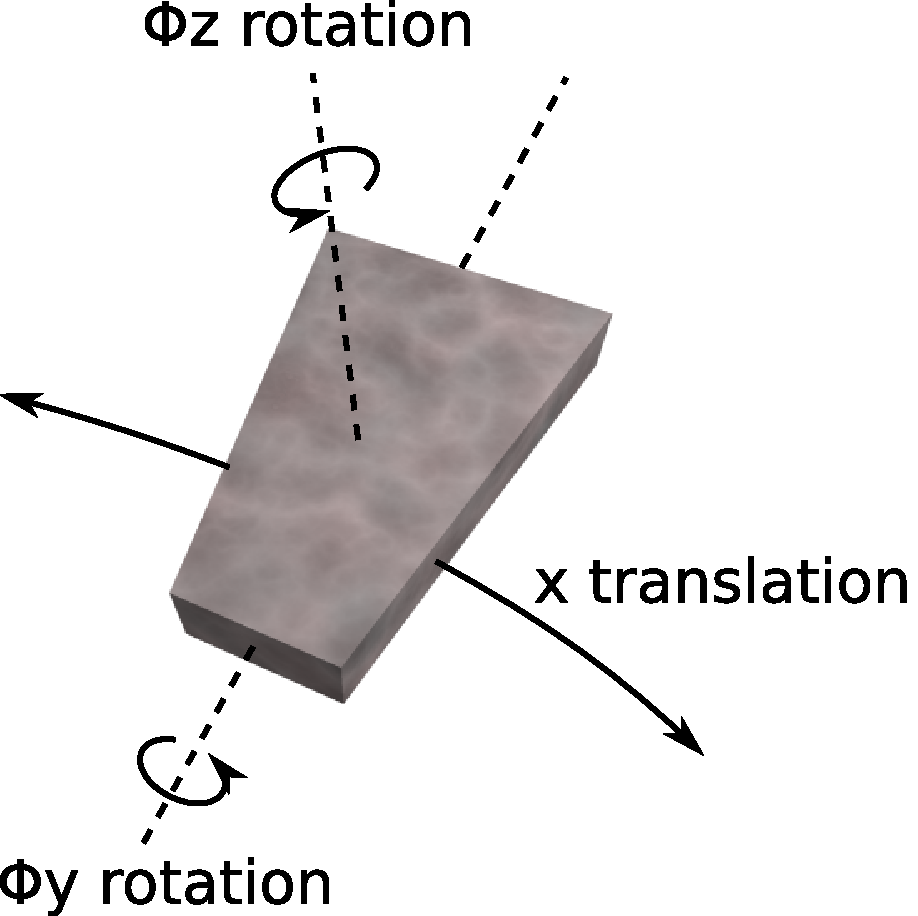
\includegraphics[width=\linewidth]{csc_coordinates2.pdf}}
\column{0.75\linewidth}

\vspace{-0.5 cm}
\begin{itemize}
\item In-practice accessible parameters are $\delta_x$, $\delta_{\phi_y}$, and $\delta_{\phi_z}$, the same as in the Overlaps procedure
\item Attempts to align others in MC yield poor resolution {\scriptsize (but with the right dependence on $R$)}
\item Complimentary to hardware's best parameters
\end{itemize}
\end{columns}
\end{frame}

\begin{frame}
\frametitle{Predicted ``Baseline'' resolution}
\begin{itemize}
\item Putting together all of the updated algorithms, MC alignment accuracy is (for 50~pb$^{-1}$, no tracker misalignment):
\end{itemize}

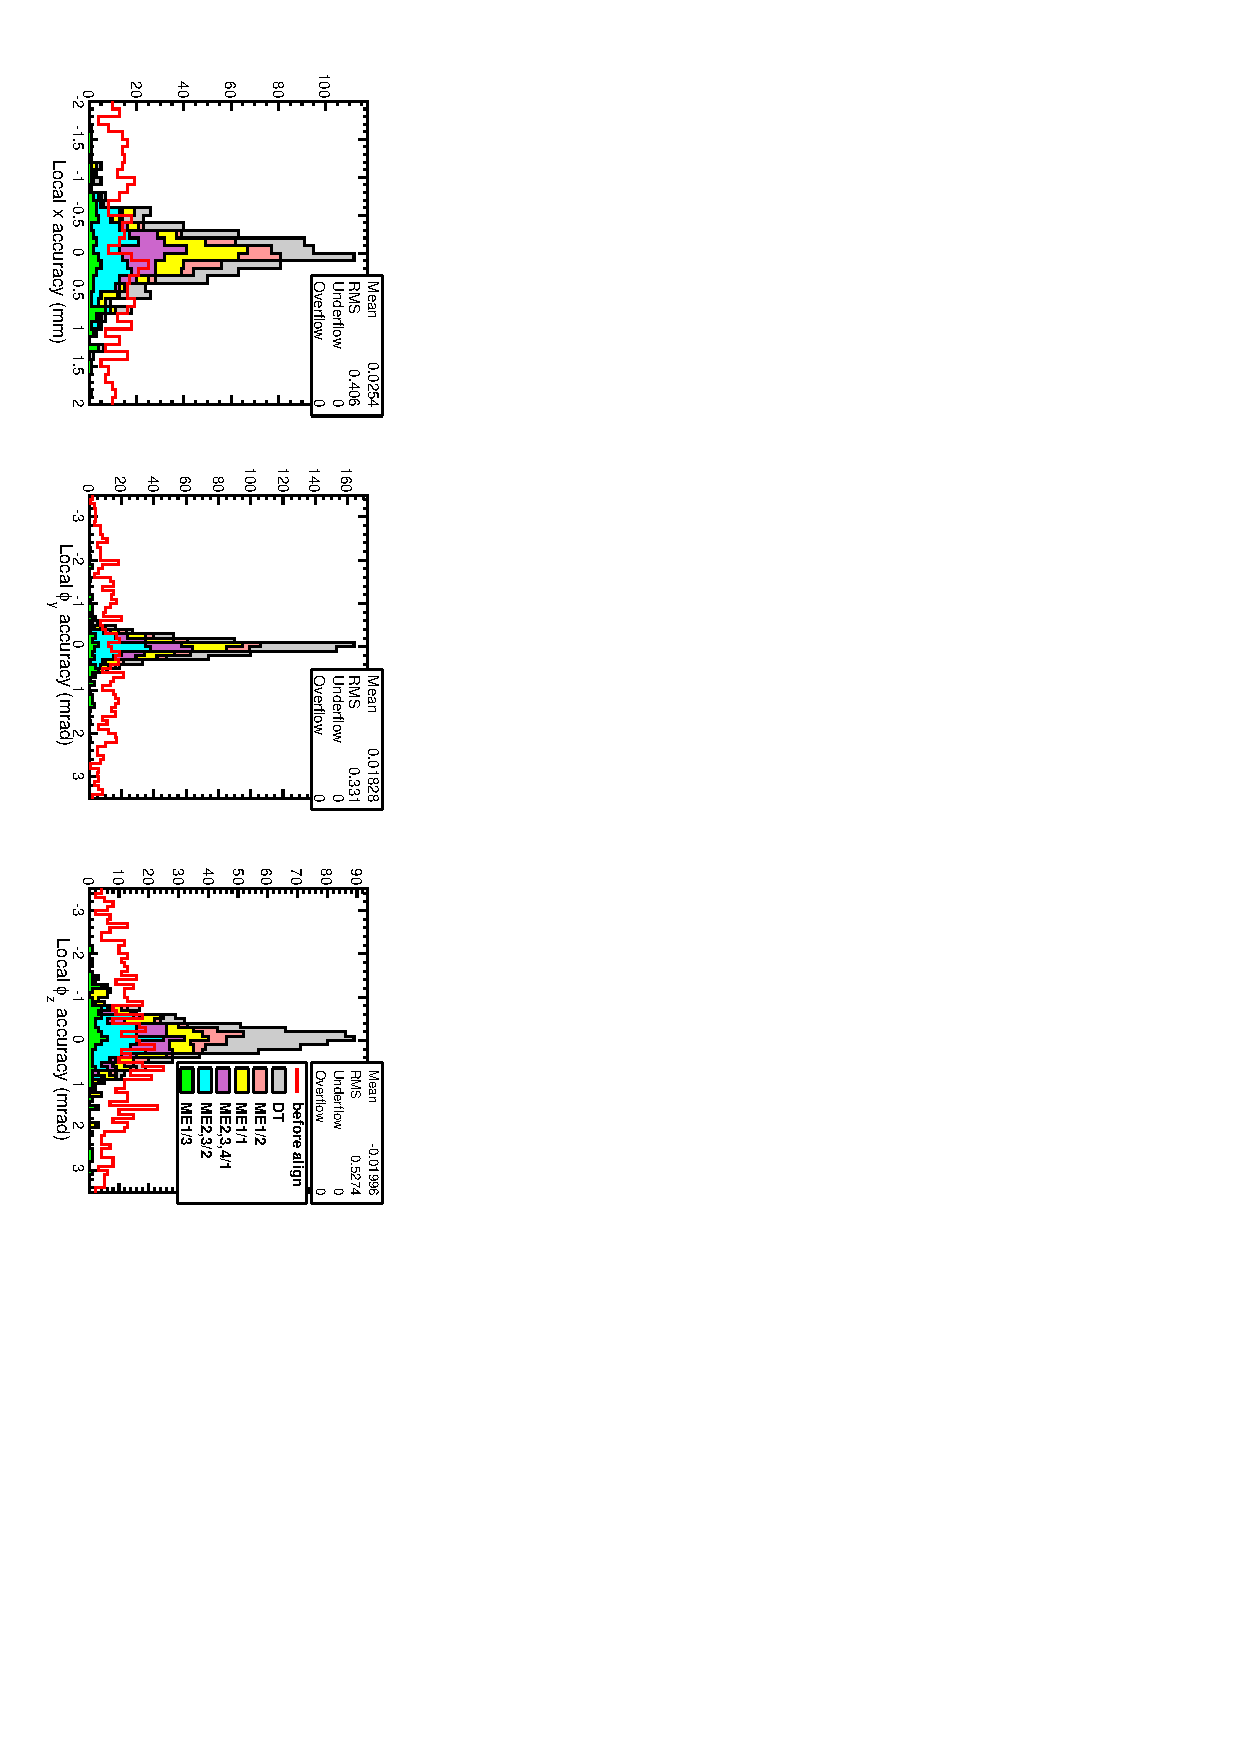
\includegraphics[height=\linewidth, angle=90]{mc_cscresolution.pdf}

\begin{center}
\scriptsize
\renewcommand{\arraystretch}{1.2}
\begin{tabular}{c c c c}
& $x$ ($\mu$m) & $\phi_y$ (mrad) & $\phi_z$ (mrad) \\\hline
DT & 430 & 0.21 & 0.31 \\
ME1/1 & 350 & 0.22 & 0.70 \\
ME1/2 & 180 & 0.24 & 0.37 \\
ME1/3 & 740 & 0.93 & 1.07 \\
ME2,3,4/1 & 250 & 0.17 & 0.47 \\
ME2,3/2 & 380 & 0.20 & 0.35 \\\hline
everything & 400 & 0.33 & 0.53
\end{tabular}
\end{center}
\end{frame}

\begin{frame}
\frametitle{Data-driven test of CRAFT $p_T$}

\begin{itemize}
\item Split $p_T \gtrsim 200$~GeV cosmic rays into upper and lower halves, refit each half independently and compare the results
\item Two track-fits for each cosmic ray: any mismatch is instrumental
\end{itemize}

\vspace{-0.5 cm}
\begin{columns}
\column{0.5\linewidth}
\begin{center}
\textcolor{darkblue}{Before muon alignment}

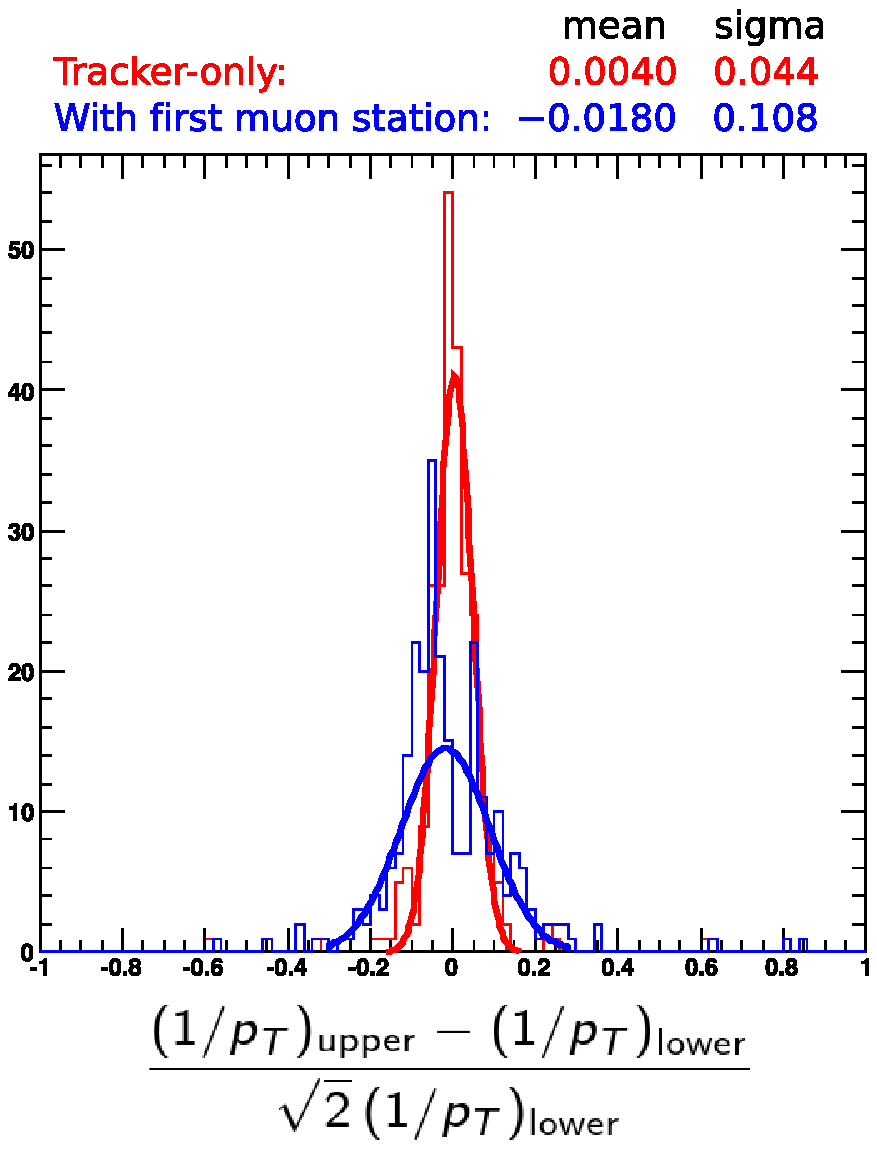
\includegraphics[width=0.9\linewidth]{without_alignment.pdf}
\end{center}
\column{0.5\linewidth}
\begin{center}
\textcolor{darkblue}{After muon alignment}

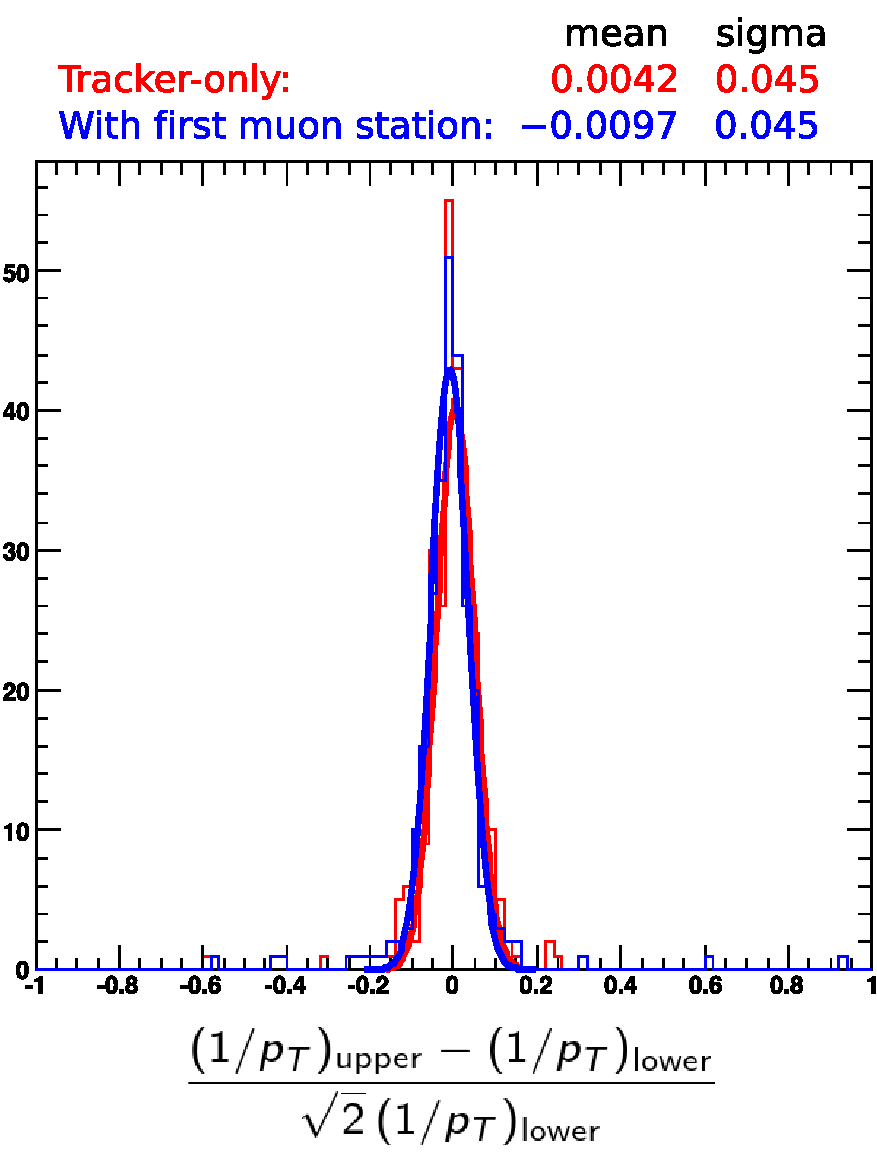
\includegraphics[width=0.9\linewidth]{with_alignment.pdf}
\end{center}
\end{columns}
\end{frame}

\begin{frame}
\frametitle{Comparison with expectations}

\begin{itemize}
\item MC resolution vs.~$p_T$ with different alignment scenarios
\item Track reconstruction method optimized by $p_T$

\mbox{\scriptsize (at high $p_T$, use only first muon station to avoid hit confusion from muon showering)\hspace{-1 cm}}
\end{itemize}

\vspace{-0.15 cm}
\begin{center}
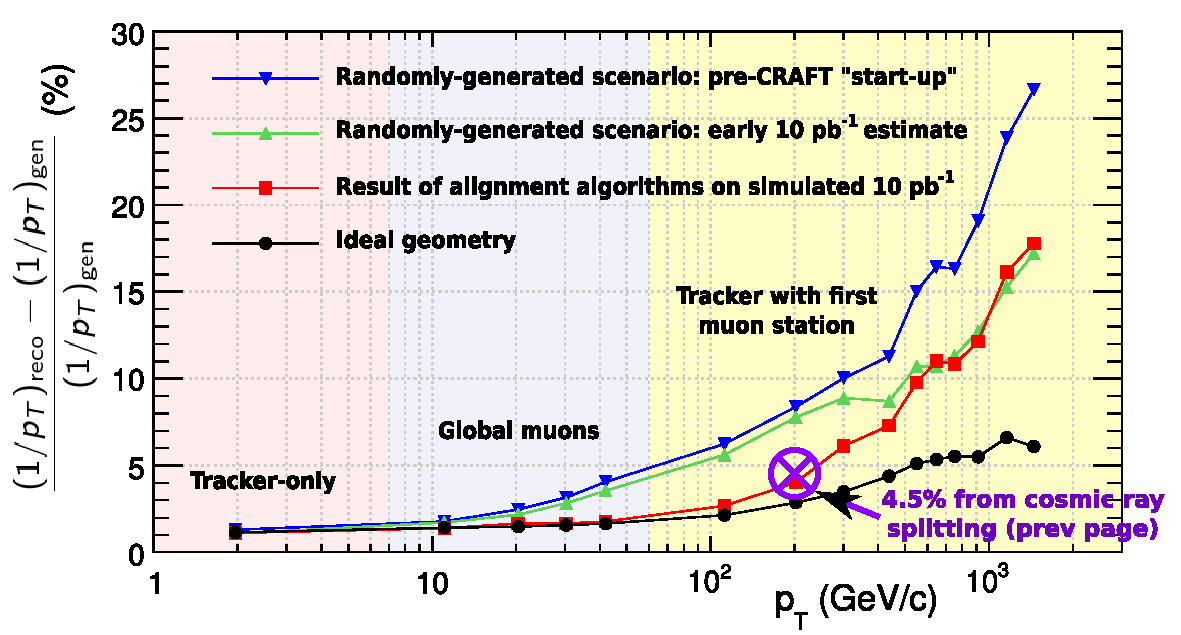
\includegraphics[width=0.9\linewidth]{curvature_resolution_cosmicpoint.pdf}
\end{center}

\vspace{-0.35 cm}
\begin{itemize}
\item \textcolor{red}{MC simulations} yield much better results than \mbox{\textcolor{darkgreen}{early estimates}\hspace{-1 cm}}
\item Cosmic ray splitting is close to MC simulations at 200~GeV
\end{itemize}
\end{frame}

\section*{3. Tracker to CSC disks}
\begin{frame}
\begin{center}
\Huge \textcolor{blue}{3. Tracker to CSC disks}
\end{center}
\end{frame}

\begin{frame}
\frametitle{3. Tracker to CSC disks}

\begin{itemize}
\item \textcolor{darkblue}{Method:} same tracker-to-muon propagation, but plot versus phi position and fit \{\textcolor{darkgreen}{const}, \textcolor{blue}{sine}, \textcolor{red}{cosine}\} to get \{\textcolor{darkgreen}{$R \phi_z$}, \textcolor{blue}{$x$}, \textcolor{red}{$y$}\} of the disk

\begin{center}
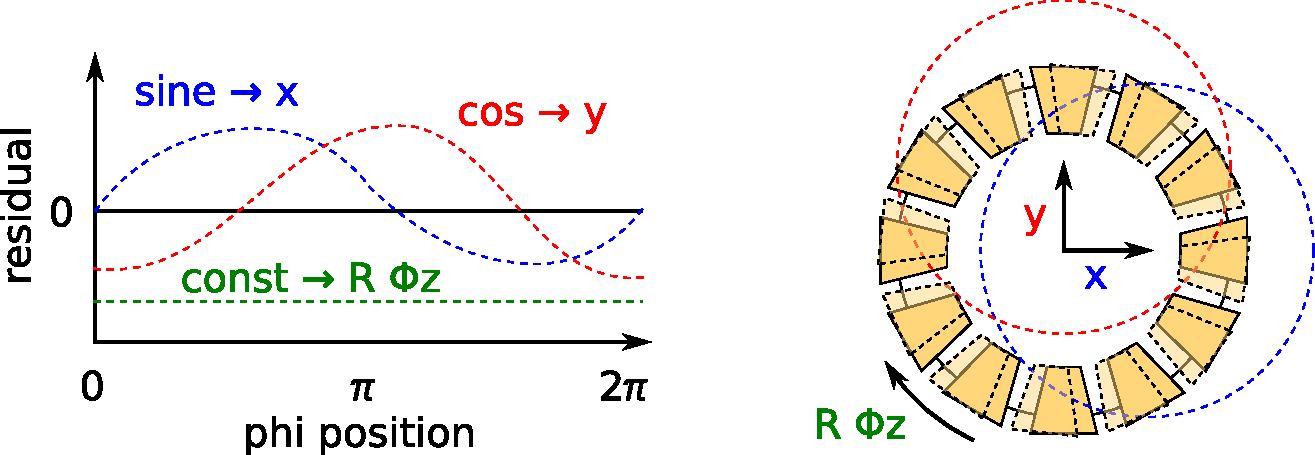
\includegraphics[width=0.9\linewidth]{tracker_disk_interpretation.pdf}
\end{center}

\item Fewer tracks are needed to align whole disks than individual chambers
\item Necessary as final step after Overlaps (internal ring alignment)
\item The following are first investigations; there are unsolved issues
\end{itemize}
\end{frame}

\begin{frame}
\frametitle{Comparison with survey (1/2)}
\begin{itemize}
\item Strip-only residuals versus phi position
\item \textcolor{blue}{Blue scale is the 2-D histogram}, black points are bin-by-bin averages
\item \textcolor{red}{Red line is a fit to the residuals}, \textcolor{darkgreen}{green line is {\it adjusted} survey}
\item Important: residuals are relative to tracker and original survey
  is relative to cavern, so we adjust survey to fit cavern to tracker
\begin{itemize}
\item \{YE$-$2, $-$1, $+$1, $+$2\} $\times$ 3 DOF is reduced to $3\times 3$ parameters
\item only meaningful to compare relative differences between rings (next page), rather than one ring alone, because of the fit
\end{itemize}

\end{itemize}
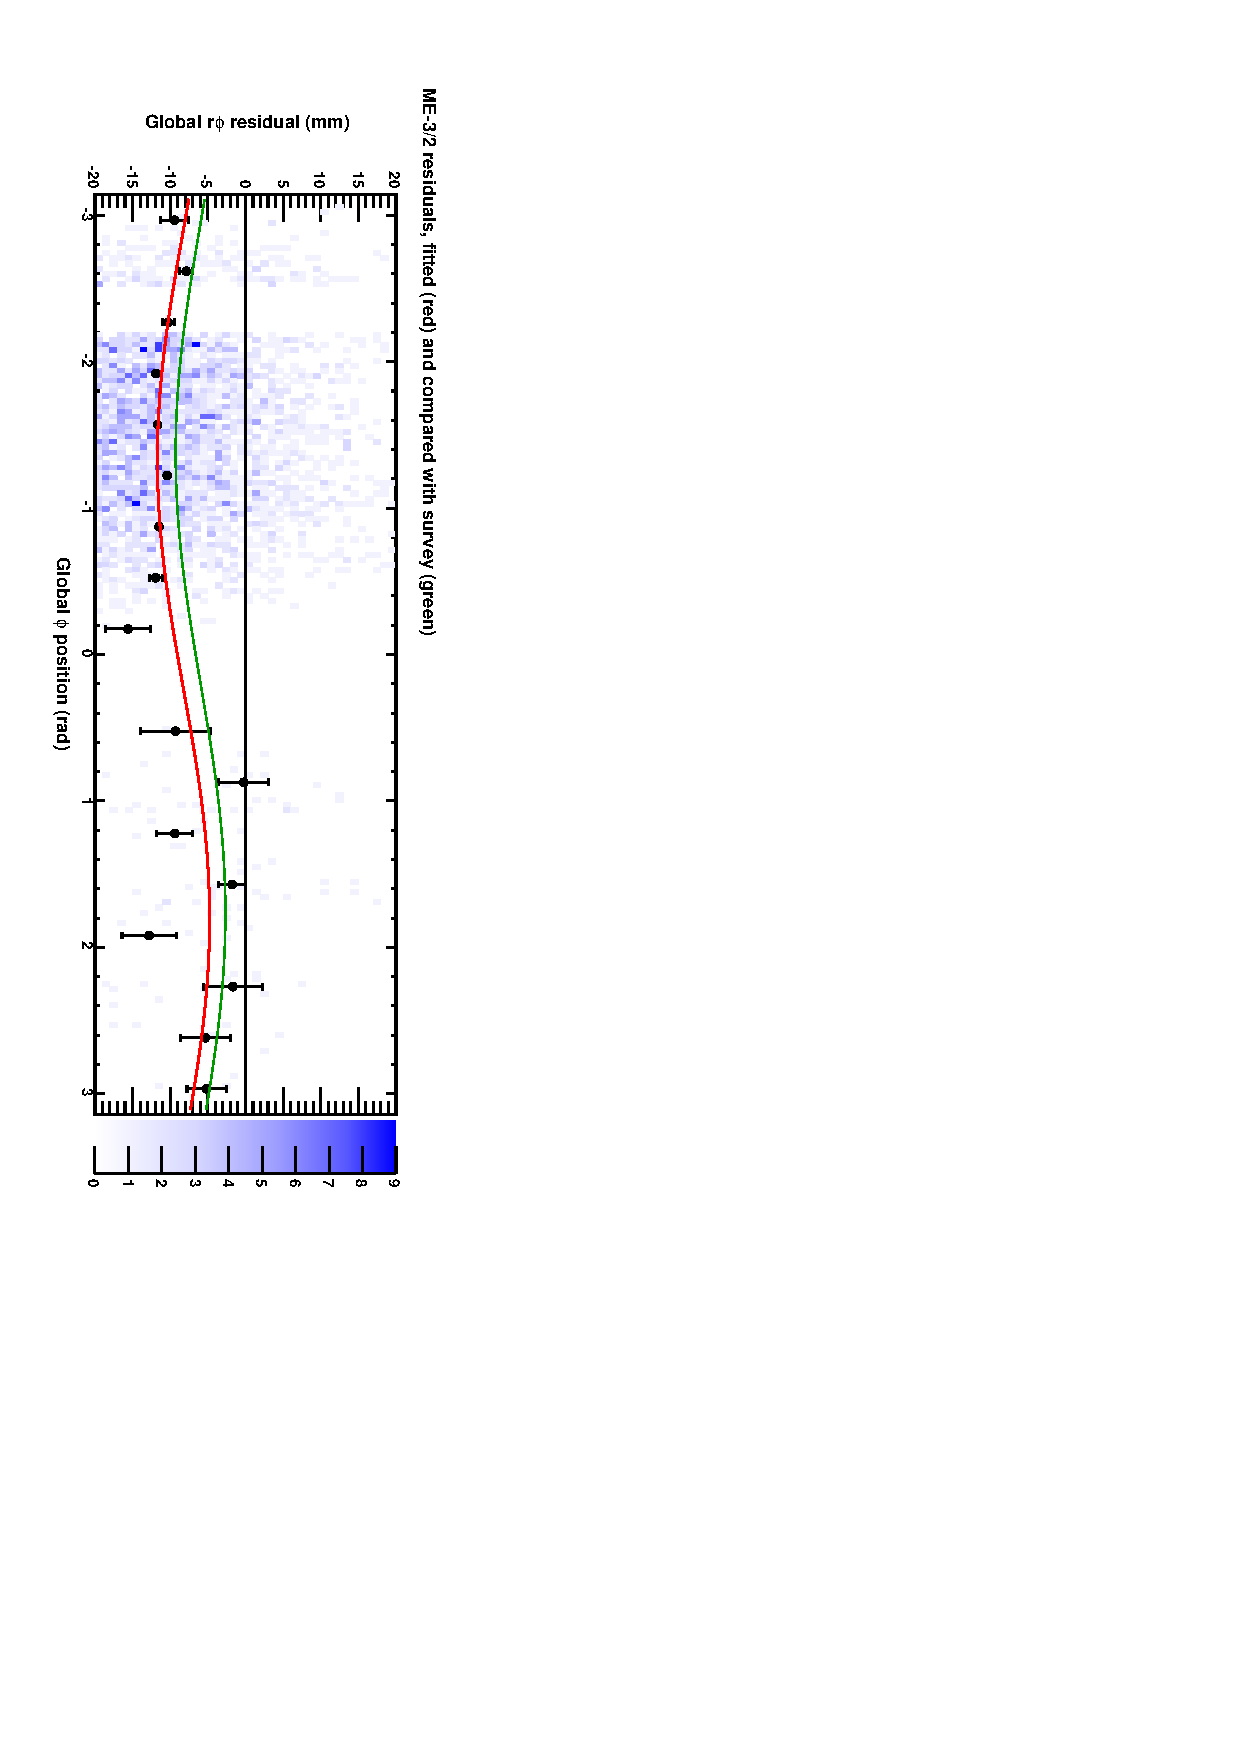
\includegraphics[height=\linewidth, angle=90]{datacsc_survey_mem32.pdf}

\scriptsize \hfill (pre-adjustment) survey data from R.~Goudard
\end{frame}

\begin{frame}
\frametitle{Comparison with survey (2/2)}

\begin{columns}
\column{0.5\linewidth}

ME$-$1/2

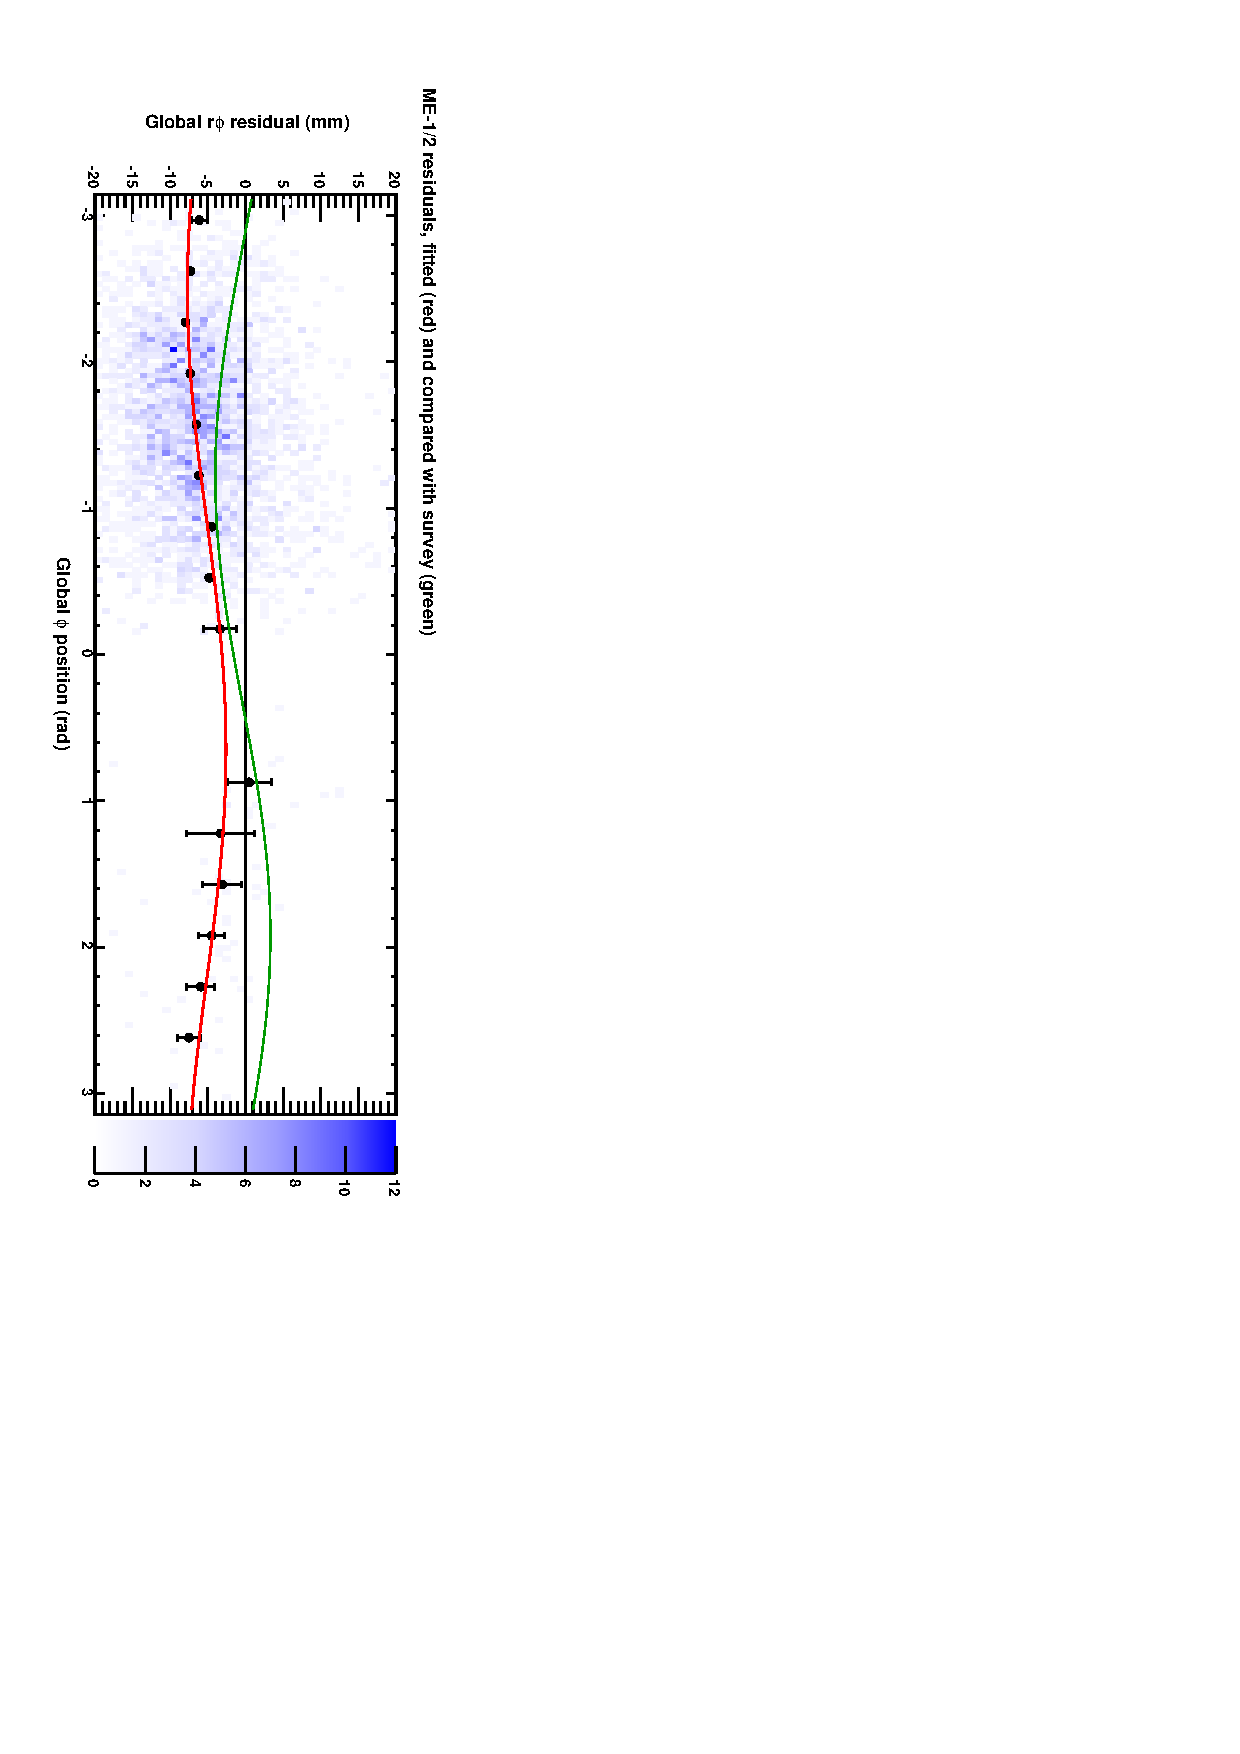
\includegraphics[height=\linewidth, angle=90]{datacsc_survey_mem12.pdf}

ME$-$2/2

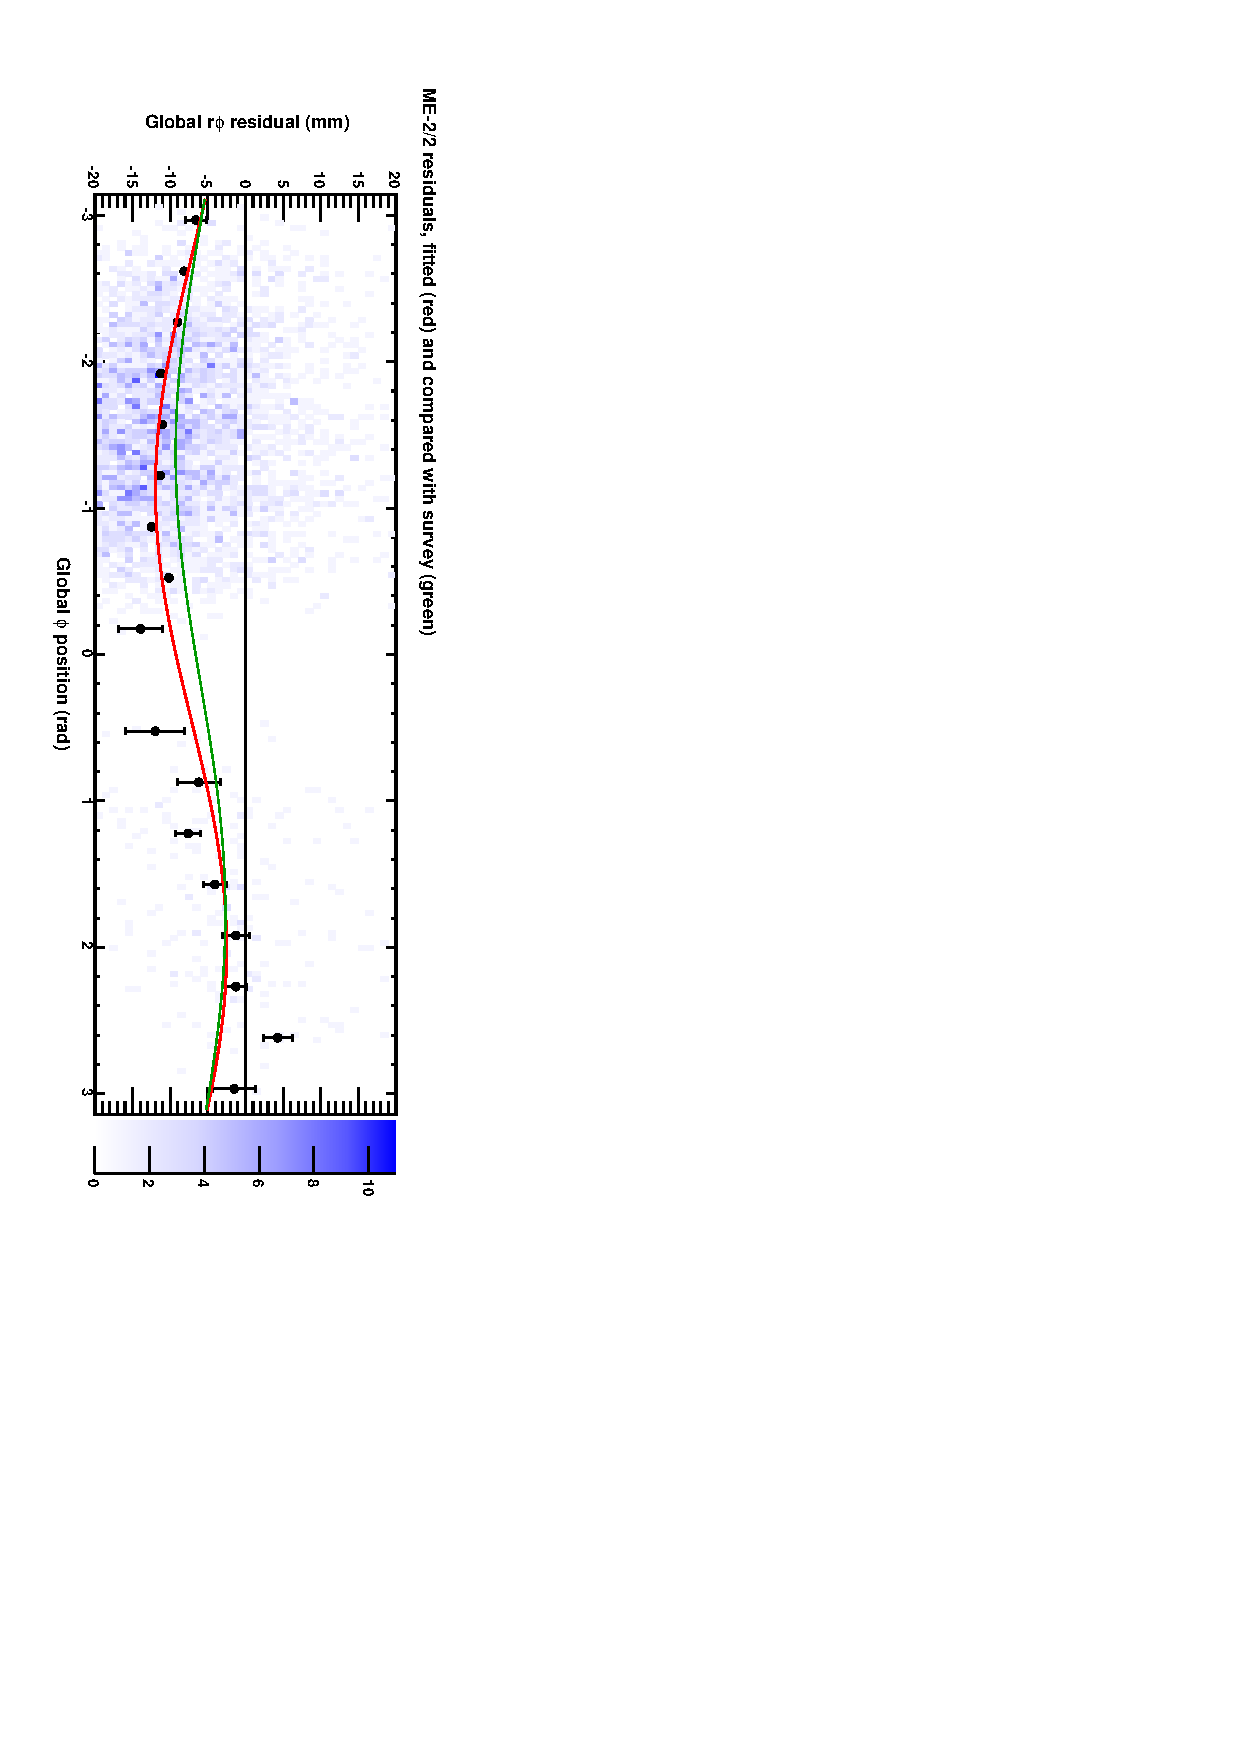
\includegraphics[height=\linewidth, angle=90]{datacsc_survey_mem22.pdf}

ME$-$3/2

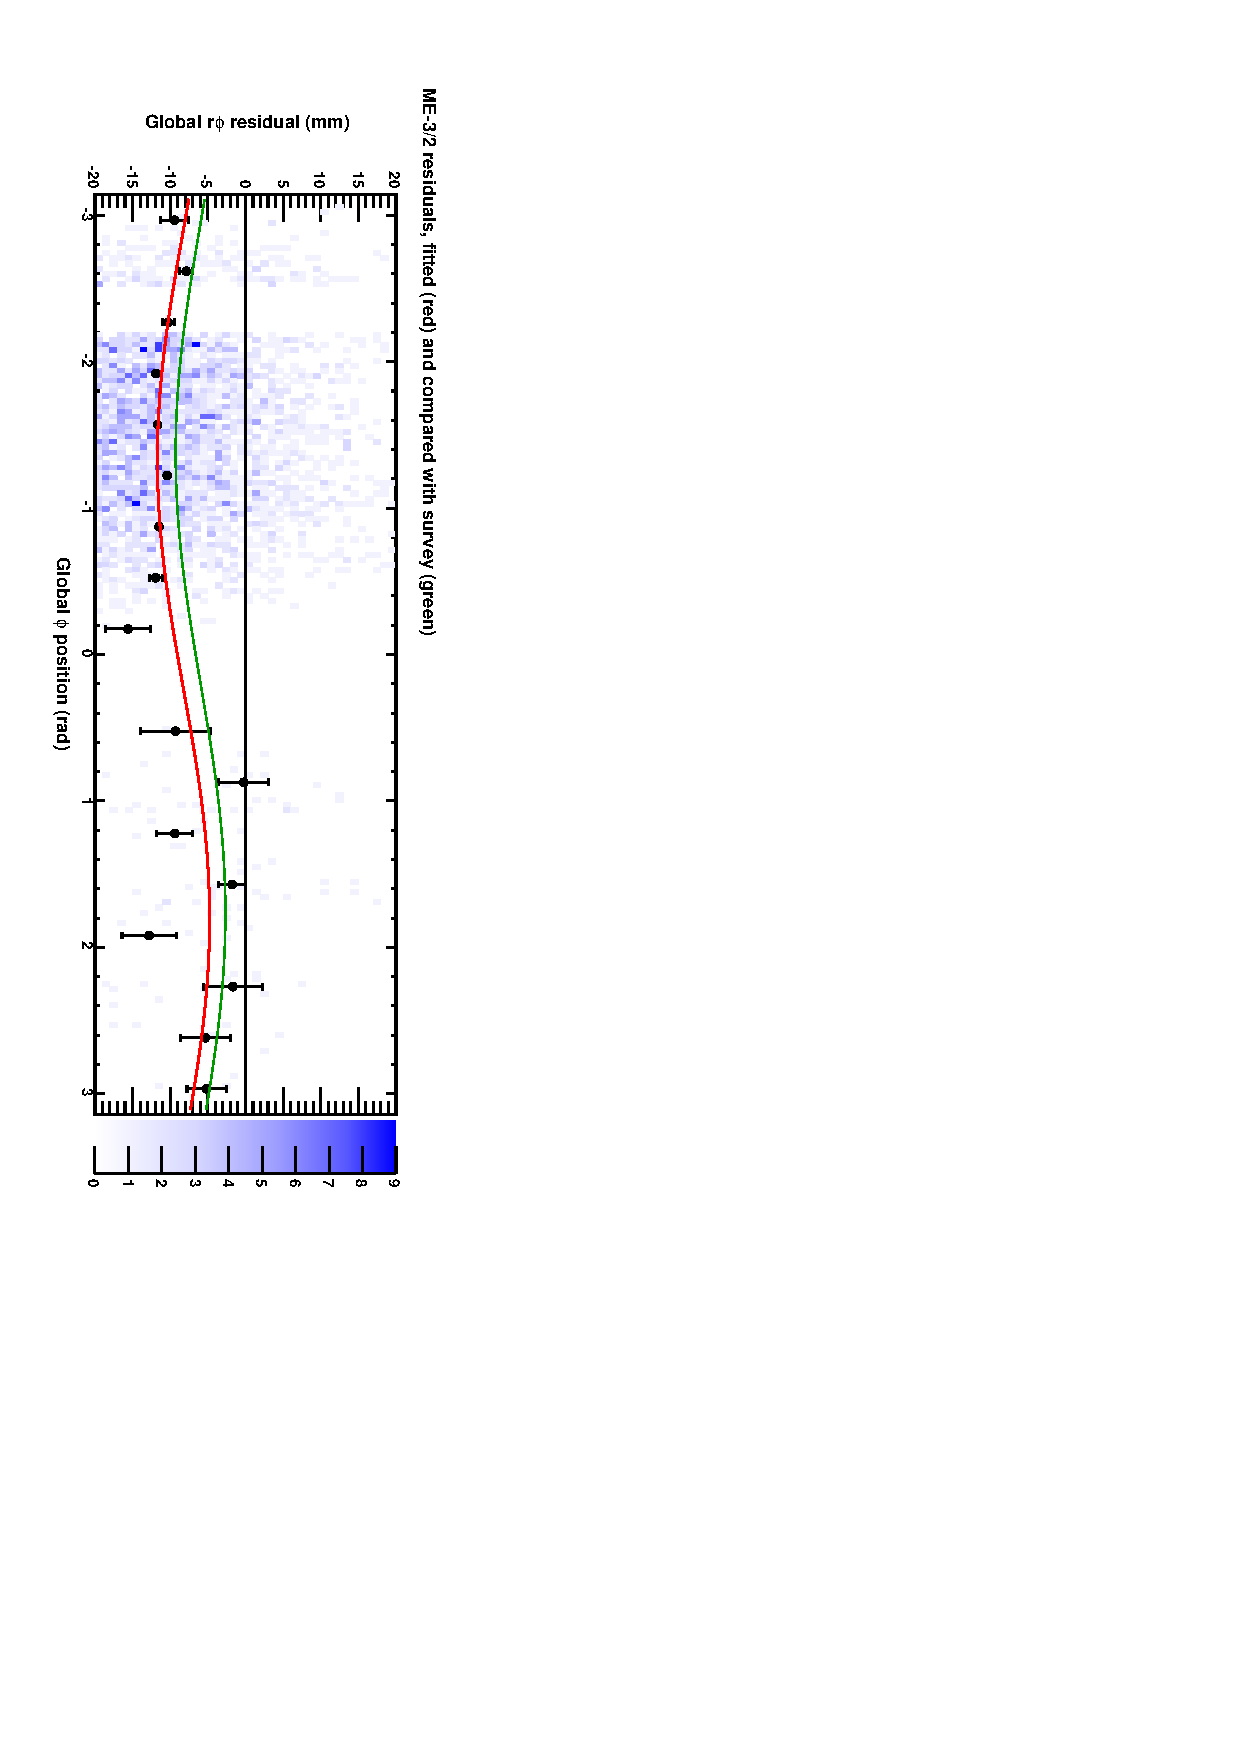
\includegraphics[height=\linewidth, angle=90]{datacsc_survey_mem32.pdf}

\column{0.5\linewidth}

ME$+$1/2

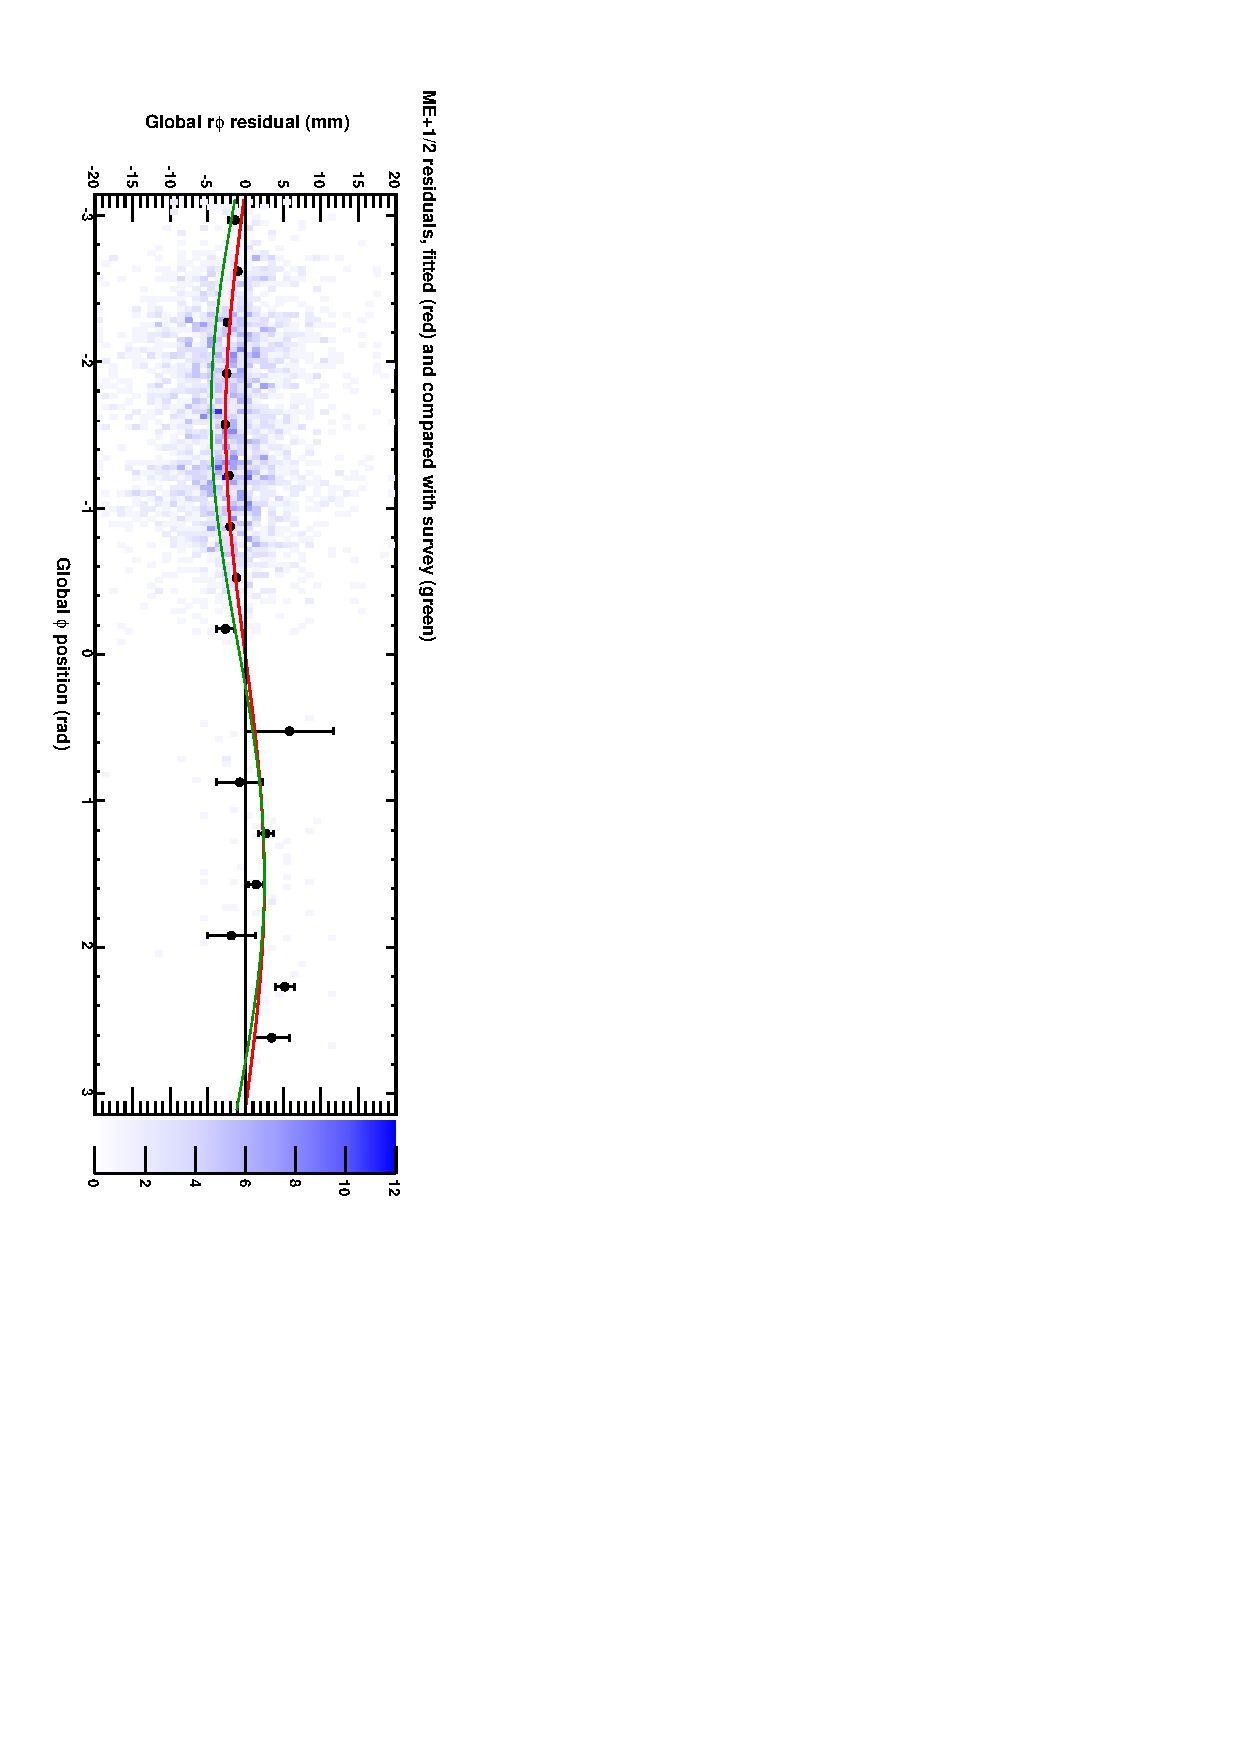
\includegraphics[height=\linewidth, angle=90]{datacsc_survey_mep12.pdf}

ME$+$2/2

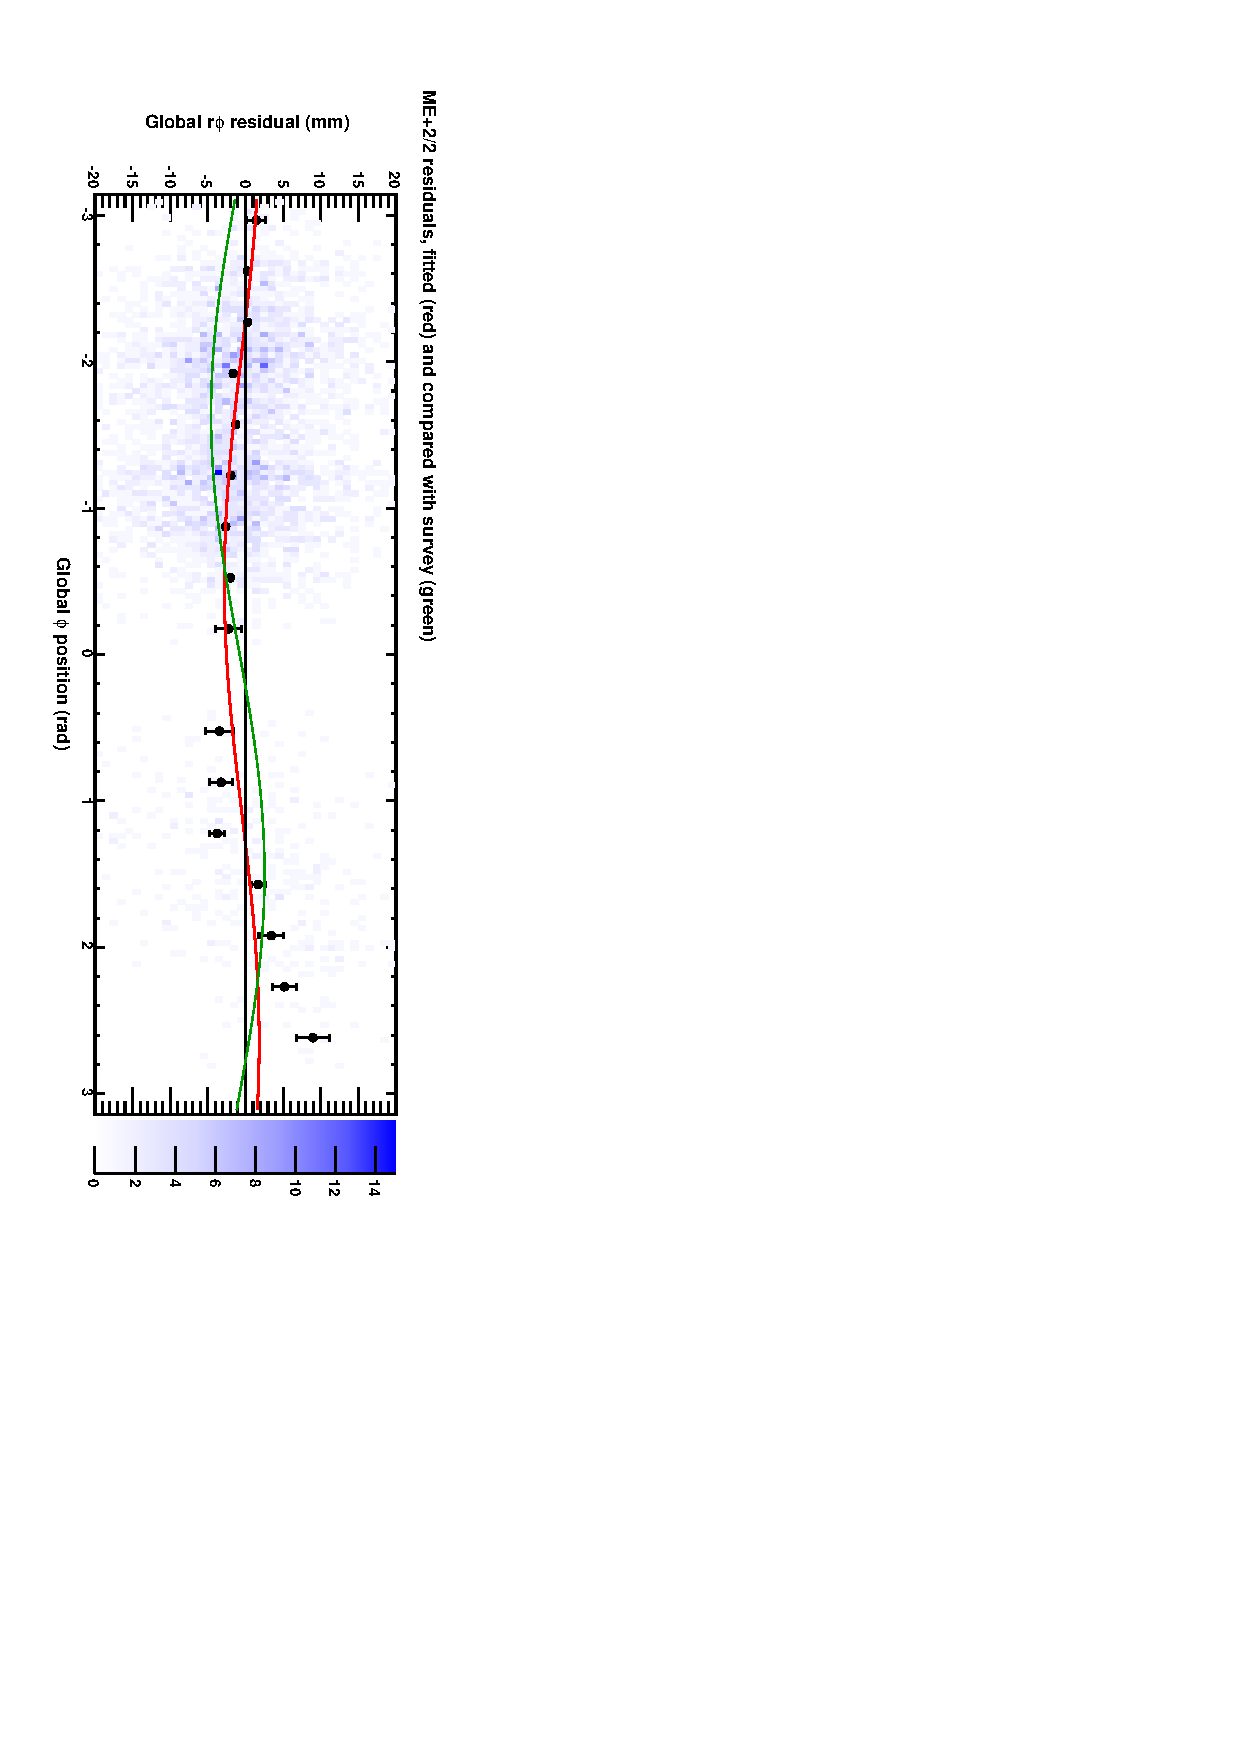
\includegraphics[height=\linewidth, angle=90]{datacsc_survey_mep22.pdf}

ME$+$3/2

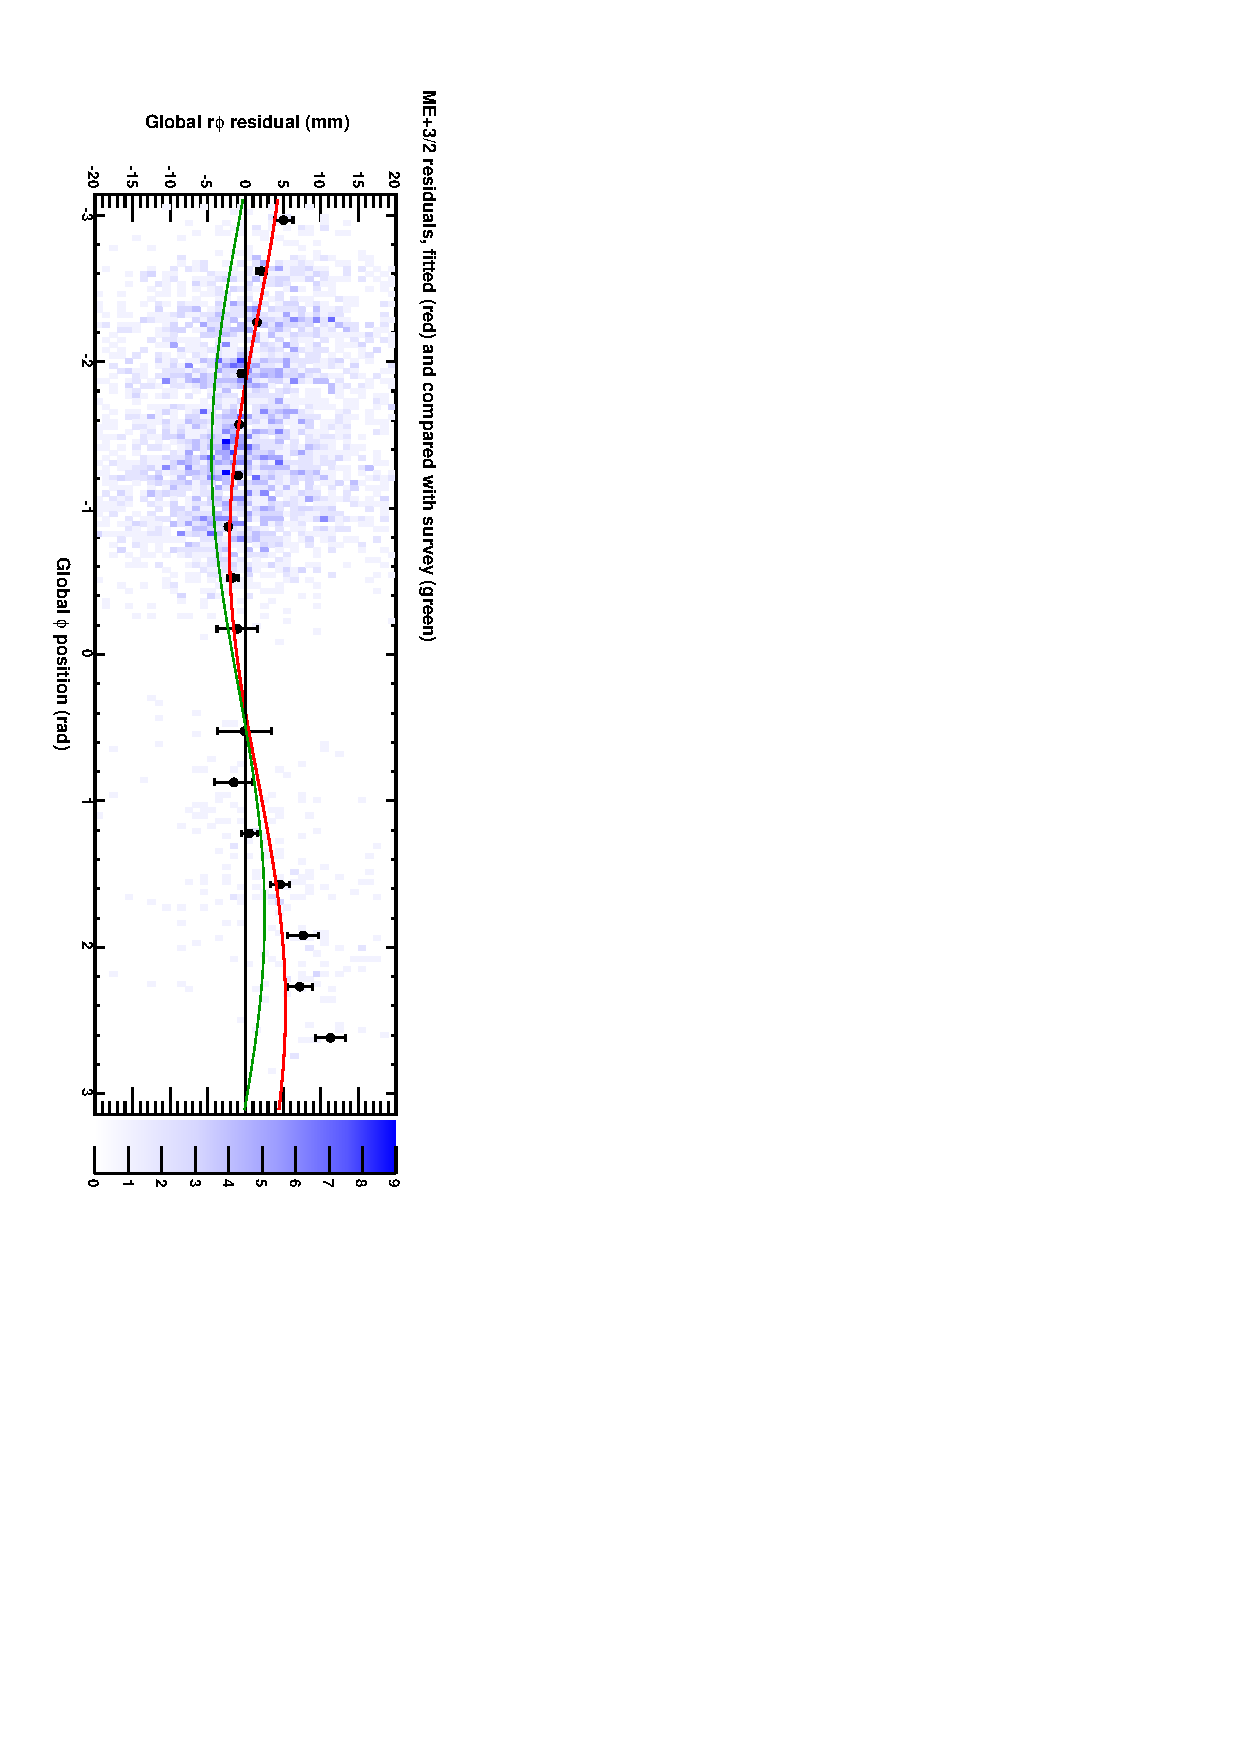
\includegraphics[height=\linewidth, angle=90]{datacsc_survey_mep32.pdf}

\end{columns}

\vfill
\begin{itemize}
\item Millimeter-level disagreement between residuals and survey
\item But ME$-$2, $-$3 and $+$2, $+$3 residuals agree with each other: good!
\end{itemize}
\end{frame}

\begin{frame}
\frametitle{Redundant binning}

\begin{itemize}\setlength{\itemsep}{0.25 cm}
\item We also have $d(r\phi)/dz$ angle residuals
\item Bin them more finely than the chambers \mbox{(dashed lines are boundaries)\hspace{-1 cm}}
\item We do observe some discontinuities, \mbox{indicating real $\phi_y$ misalignments\hspace{-1 cm}} \\ between chambers
\item Few-mrad is the same misalignment scale that was observed by beam-halo
\end{itemize}

\vspace{0.5 cm}
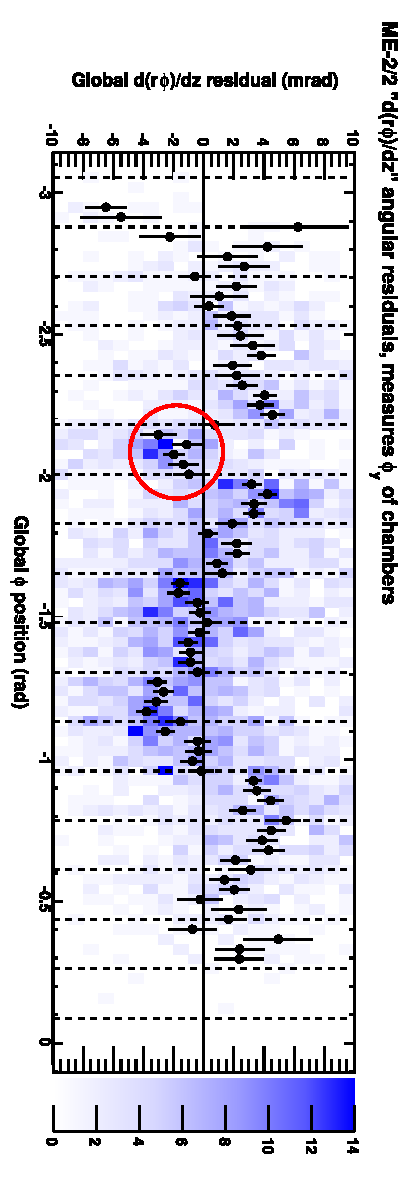
\includegraphics[height=\linewidth, angle=90]{datacsc_phiy_misalignment.pdf}
\end{frame}

\begin{frame}
\frametitle{Comparison with beam-halo}
\begin{itemize}\setlength{\itemsep}{0.25 cm}
\item Difficult to actually compare tracker-to-disk and beam-halo directly, because very few cosmic rays connect ME$-$2/1 with the tracker
\item Nevertheless, we can try: these are $\phi_y$ with \textcolor{red}{beam-halo} overlaid

\begin{center}
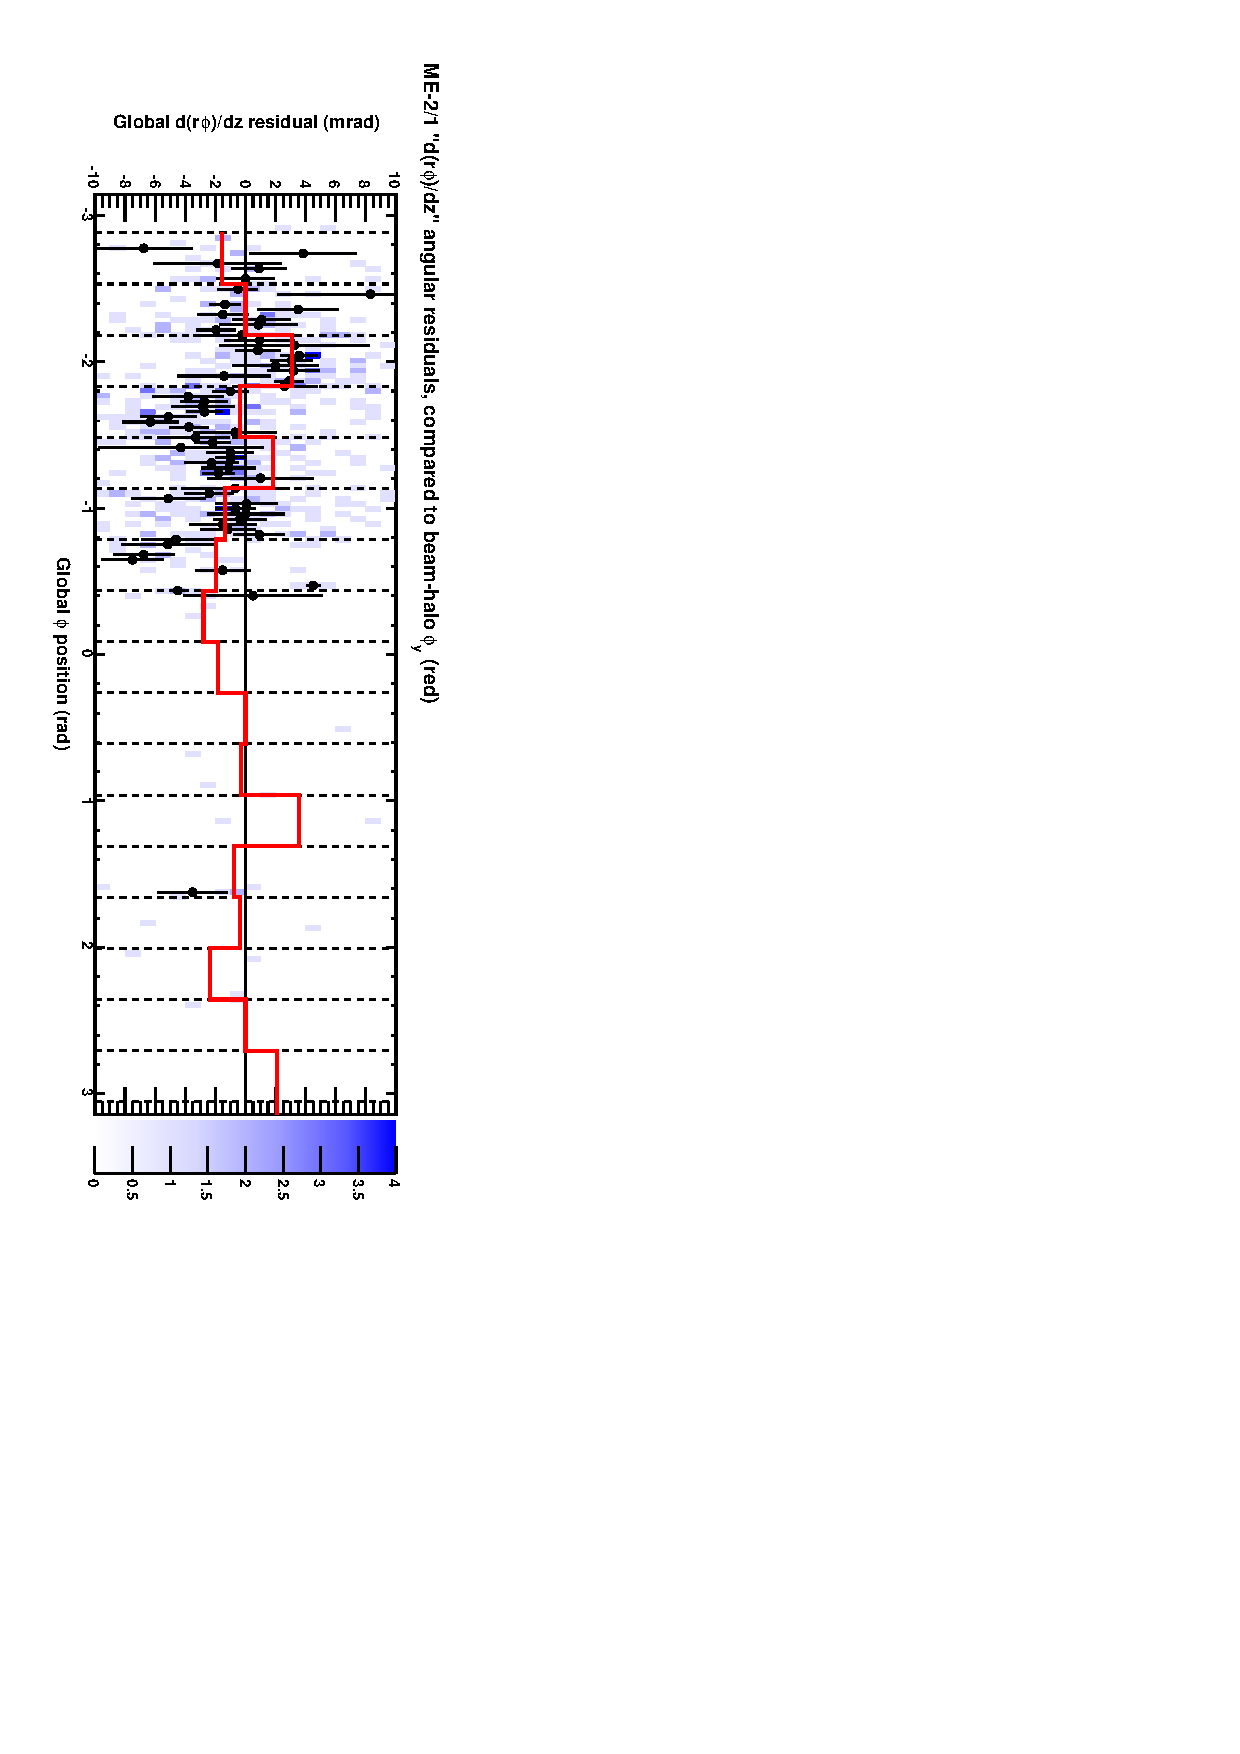
\includegraphics[height=\linewidth, angle=90]{datacsc_phiy_andbeamhalo.pdf}
\end{center}

\item To allow for tracker distortions and propagator errors, we can focus on the discontinuities at the chamber boundaries
\item The discontinuities do not agree in detail with beam-halo: can form an argument that chambers have rotated between \mbox{$\vec{B}=0$ and CRAFT\hspace{-1 cm}}
\end{itemize}
\end{frame}

\begin{frame}
\frametitle{How does it look in MC?}

\begin{itemize}\setlength{\itemsep}{0.25 cm}
\item Collisions MC (5~pb$^{-1}$): tracks uniform in $\phi$ but not more numerous
\item Much easier to fit const $+$ sine $+$ cosine, accurate results
\item Roughly the same widths
\item Cosmic-ray MC (full sample): zero tracks {\scriptsize (probably a generator-level cut)}
\end{itemize}

\vspace{0.5 cm}
\includegraphics[height=\linewidth, angle=90]{mccsc_example_5pb.pdf}
\end{frame}

\begin{frame}
\frametitle{MC disk-fitting study}
\begin{itemize}
\item With $\phi$-symmetric collisions, how much data do we need to align the disks?
\item Includes residual misalignments after CSC Overlaps alignment (assuming same resolution as 2008)
\item Independent samples scale with $\sqrt{N}$
\end{itemize}

\includegraphics[height=0.5\linewidth, angle=90]{mccsc_diskstats_xy.pdf}
\includegraphics[height=0.5\linewidth, angle=90]{mccsc_diskstats_phiz.pdf}
\end{frame}

\section*{Conclusions}

\begin{frame}
\frametitle{Timeline for beam}
\scriptsize
\begin{itemize}
\item Now and CRAFT-2009
\begin{itemize}
\item \scriptsize validate cosmic ray tracker-to-disk procedures with CRAFT-2008 \mbox{and -2009\hspace{-1 cm}}
\item \scriptsize automate all procedures and monitoring for CRAFT-2009, then simply run them
\end{itemize}

\item Month of beam-halo only
\begin{itemize}
\item \scriptsize re-run beam-halo procedure on new samples
\item \scriptsize kludge incomplete rings if necessary
\item \scriptsize any corrections needed for $\vec{B} \ne 0$?
\item \scriptsize one-time layer alignment with full dataset \\ {\scriptsize (low-statistics 2008 pilot study on right)}
\end{itemize}

\vspace{-2.90 cm}
\hfill \includegraphics[width=0.3\linewidth]{layer_hist.pdf}

\vspace{-1.20 cm}
\mbox{ }

\item First collisions: 5~pb$^{-1}$
\begin{itemize}
\item \scriptsize run Overlaps procedure on collisions data, compare with beam-halo result
\item \scriptsize use tracker-to-disk method to connect internally-aligned rings to tracker
\end{itemize}

\item Later collisions: 50~pb$^{-1}$
\begin{itemize}
\item \scriptsize run Baseline procedure with same tracks: do they agree?  If not, do track-by-track comparisons to diagnose the problem
\item \scriptsize do collisions alignments agree with cosmic rays in the barrel?
\item \scriptsize when all of these are resolved, we will have a physics-quality alignment!
\end{itemize}
\end{itemize}
\end{frame}

%% \section*{First section}
%% \begin{frame}
%% \begin{center}
%% \Huge \textcolor{blue}{First section}
%% \end{center}
%% \end{frame}

\begin{frame}
\frametitle{Conclusions}
\begin{itemize}\setlength{\itemsep}{0.5 cm}
\item We have used 2008 beam-halo and CRAFT samples to be as prepared as possible for aligning with collisions
\item Beam-halo demonstration vetted our knowledge of local aspects of
  alignment (such as CSC strip pitch angle); CRAFT wheel $-$1, 0, $+$1 alignment tests
  propagation of tracks over long distances through iron and imperfect
  magnetic fields
\item We have produced and uploaded track-based constants for most
  barrel chambers, and for endcap disk positions, though our understanding
  of the latter can be significantly improved
\item We know what issues we'll need to work on, at what time, in the
  LHC start-up process
\end{itemize}
\label{numpages}
\end{frame}

\end{document}
